\documentclass[fleqn]{sig-alternate}
%\documentclass{vldb}
%\documentclass[10pt,conference,letterpaper]{IEEEtran}
\usepackage{amsmath}
\usepackage{multicol}
\usepackage{algorithm}
\usepackage{algorithmic}
%\usepackage{hyperref}%[colorlinks, citecolor=blue, hyperindex]
\usepackage{graphicx}
\usepackage{url}
\usepackage{color}
%\usepackage{algorithm2e}
%\usepackage{subfigure}
\graphicspath{{figures/}}

%\usepackage{caption}
\begin{document}
\title{Clustering Concepts for Semantic Similarity between Terms}
\author{%
% author names are typeset in 11pt, which is the default size in the author block
{Peipei Li{\small $~^{\#*1}$}, Haixun Wang{\small $~^{*2}$}, Kenny Zhu{\small $~^{\dag3}$}, Zhongyuan Wang{\small $~^{*4}$}, Xindong Wu{\small $~^{\#5}$} } %
% add some space between author names and affils
\vspace{1.6mm}\\
\fontsize{10}{10}\selectfont\itshape
$~^{\#}$Hefei University of Technology\\
%Hefei, China\\
\fontsize{9}{9}\selectfont\ttfamily\upshape
$~^{1}$v-pli@microsoft.com\\
\fontsize{9}{9}\selectfont\ttfamily\upshape
$~^{5}$xwu@uvm.edu
% add some space between email and affil
\vspace{1.2mm}\\
\fontsize{10}{10}\selectfont\rmfamily\itshape
$~^{*}$Microsoft Research Asia\\
\fontsize{9}{9}\selectfont\ttfamily\upshape
$~^{2}$haixunw@microsoft.com\\
\fontsize{9}{9}\selectfont\ttfamily\upshape $~^{3}$Zhy.Wang@microsoft.com\\
\fontsize{10}{10}\selectfont\rmfamily\itshape
$~^{\dag}$Shanghai Jiao Tong University\\
%, Shanghai, China\\
\fontsize{9}{9}\selectfont\ttfamily\upshape
$~^{4}$kzhu@cs.sjtu.edu.cn\\
}
\maketitle
\begin{abstract}
Semantic similarity between terms is essential for a variety of text analytics and text understanding applications. To measure the semantic similarity between terms, there are mainly two approaches, namely the knowledge resource based and the distributional context based methods. However, these approaches are more suitable for the measuring of the semantic similarity between words, and the scalability problems due to manual tagging and corpora dependency and availability also limit their applicability.
Contrary to existing techniques, we propose a lightweight and effective approach for the semantic similarity between terms with any multi-word expression. To extend the data coverage, we first selectively collect the semantic contexts of terms from the Web data. Second, to measure the semantic similarity between terms accurately, we introduce the clustering approach to identify potential senses of terms instead of manually tagging, and then compare the term's sense based contexts to get the semantic similarity between terms. Extensive studies demonstrate our approach can accurately measure the semantic similarity between terms with multi-word expressions and ambiguity. The pearson correlation coefficient can be improved by 0.5 at least compared to the state-of-the-art approaches for the semantic similarity measurement between terms. Meanwhile, our approach is much more efficient and can be applied on measuring semantic similarity with a large scale of pairs.
\end{abstract}

% , and knolnumber
  % of conceptualization In order Meanwhile, in a massive corpus, a
  % substantial fraction of extractions appear infrequently. It is hence
  % a challenge for traditional information extraction techniques to
  % assess these large scale sparse extractions. Motivated by this
  % challenge, this paper shows how to assess the correctness of sparse
  % extractions by utilizing the semantic context-based assessment
  % approach. In our proposed method, we adopt three different semantic
  % contexts. Firstly, we use the conceptualization method to get a set
  % of representative concepts from the sentences as the
  % context. Secondly, we extract the attributes as the
  % context. Thirdly, we collects the isA concepts as the context. In
  % terms of these semantic contexts, we implement a similarity
  % evaluation to rank extractions by the likelihood that they are
  % correct. Lastly, we apply our approach into the Hearst pattern
  % database of Probase, which contains 2425558 concepts and 15805500
  % extractions extracted using Hearst patterns from 1.68 billion web
  % pages and two years' worth of Microsoft Bing's search
  % log.


% A category with the (minimum) three required fields
%\category{H.4}{Information Systems Applications}{Miscellaneous}
%A category including the fourth, optional field follows...
%\category{D.2.8}{Software Engineering}{Metrics}[complexity measures, performance measures]

%\terms{Theory}

%\keywords{ACM proceedings, \LaTeX, text tagging} % NOT required for Proceedings

\section{Introduction}
%\KZ{What's the definition of term? What is term similarity? Explain briefly the diff between
%similarity and relatedness. Why is term similarity important?}
%\KZ{One problem is that we don't handle verbs or adjectives. We
%need to point this out either in the title or somewhere here.}

Measuring semantic similarity between terms is a fundamental problem
in lexical semantics \cite{Budanitsky:2006} and it finds many
applications in web and document search \cite{WangLWZ12:Concept}, question and answer systems,
and other text analytics and text understanding scenarios.  By {\em
  terms}, we mean either single words or multi-word expressions
(MWEs).
%{\color{red}in this paper, we refer terms as the collective
%concepts and entities}.
We say two terms are semantically similar, if their
meanings are close, or the concept or object that they represent share many common attributes.  For example, ``emerging markets'' and
``developing countries'' are similar because their semantic contents (the subset of countries) are very similar. Another example, ``Google'' and
``Microsoft'' are similar because they are both software companies. %  and
% as a software company, they share a number of commonalities.
However, ``car'' and ``journey'' are not semantically similar but {\it related} because ``car'' is a transport means for
  the activity ``journey''. Specifically, semantic
similarity is defined by some measure of {\em distance} between two terms on an isA taxonomy.
%which organizes terms by {\em synonymy} and {\em hypernumy} relations.
% Such distance can be either a naive metric of number of distinct edges
% (hops) between two nodes on the taxonomy graph, or more sophisticated
% statistical measures.
It is clear that ``car'' and ``journey'' are quite far away from each other in an isA taxonomy from WordNet as shown in Figure~\ref{fig:tree}.
Semantic similarity is a more specific relationship and is much harder to model than {\em relatedness} (which can be modeled by term
co-occurrence).
% In this paper, we are concerned
% with the efficient computation of semantic similarity between two
% terms.
\begin{figure}[th]
 \centerline{
 \includegraphics[width=0.5\textwidth]{car-journey.eps}}
\caption{A fragment from WordNet showing semantic distance between ``car'' and ``journey''}
\label{fig:tree}
\end{figure}
%\KZ{Include a graph cut from wordNet that shows the distance between
%car and journey.}

%Semantic similarity is different from semantic relatedness.
% Contrary to the semantic relatedness relying on the more general relationships (e.g., part-of and the co-occurrence), semantic similarity relies on the degree of taxonomic
%likeness between concepts considering relationships such as hyponymy and hyperonymy, but most of the semantic similarity measurement methods can be adapted and generalized to deal with semantic relatedness.
%We can adapt and generalize the semantic similarity measurement methods to deal with semantic relatedness, but we cannot adapt the semantic relatedness measurement methods to deal with semantic similarity. For example, \emph{journey} and \emph{car} has a high semantic relatedness score due to the higher co-occurrences in the corpus, while its semantic similarity should be lower because they belong to the different concepts.


%\KZ{Briefly state the existing approaches. Classify them into two categories. State why they don't work for some
%examples. Use concrete examples (challenge 1-3) from the slides to
%illustrate the challenges.}
% Computing the semantic similarity between two terms is tantamount to
% computing the similarity between their {\em contexts}.
Recent work on term similarity can be roughly classified into two main categories: {\em knowledge based} and {\em corpus based}. Knowledge based
approaches rely on handcrafted resources such as thesauri, taxonomies or encyclopedias, as the context of comparison.  Most work in this space
\cite{Rada:1989, Resnik:1995, Agirre:2010} depends on the semantic isA relations in WordNet \cite{Miller1995} which is a manually curated
lexicon and taxonomy. Corpus based approaches work by extracting the contexts of the terms from large corpora and then inducing the
distributional properties of {\em words} or {\em
  n-grams}.
%{\color{red}(It also include the term co-occurrence based method)}.
Corpus can be anything from web pages, web
search snippets to other text repositories.
%For example, Google distance \cite{Cilibrasi:Google} is
%derived from the number of hits returned by the Google search engine.
%Other corpus-based measures rely on the
%content of search results or search snippets.

One significant challenge faced by the knowledge-based methods is the
limited coverage of taxonomies such as WordNet (with 155,287 words
at last count).
%Through two decades of development, the most recent release
%of WordNet (version 3.0) contains
%155,287 words organized in 117,659 synsets and 206,941 word-sense pairs.
It does not cover many proper nouns (e.g., ``Microsoft''
or ``Google''), or very popular senses (e.g., Apple the company or
Jaguar the car make). Another major restriction of WordNet is that it
primarily covers single words with only a handful of phrases or
multi-word expressions.  For example, it does not know ``General
Electric'' or ``emerging markets''.
%Thus, it is impossible for these
%WordNet-based methods to correctly compute the semantic similarity
%which involves these unknown terms or terms with unknown senses.
Consequently, the similarity between ``General Electric'' and ``GE''
is completely ignored.
%they are exactly the same thing.
%With today's fast changing world, it is just not possible for manually
%curated lexical databases like WordNet to keep up with the pace of the
%creation of new words and phrases in human languages.
%
%Meanwhile, new words are constantly being
%created on the Web as well as new senses are assigned to existing words,
%it is also costly for manually maintaining existing thesauri like
%WordNet to capture these new words and senses if not impossible.

Corpus-based approaches also face several serious limitations.
First, such measures are biased because of the indexing and 
ranking mechanisms used in search engines. 
% Unfortunately, these mechanisms are often ``commercial
% secrets'' and are opaque to outsiders.
For example when querying the term ``date''
%\footnote{sense 1: day of the month; ...; sense 8: sweet edible fruit of the
%date palm with a single long woody seed.}
or ``range''
%\footnote{sense 1: scope; ...; sense 9: stove, kitchen stove. Senses of
%``date'' and ``range'' mentioned above are annotated in WordNet.}
on Google, none of the first 100 results has anything to do with
fruits (a sense for date) or cooking stoves (a sense for range),
because these are rare senses of the two terms.
%and are considered not ``relevant'' by Google.
With such search results, it is not surprising that a corpus-based
method would think ``asian pear'' and ``date'' share very little commonality.
%and ``food processor'' and ``range'' are very different, too.
Second, some search-result oriented similarity methods require
interaction with the search engine which has high communication overhead
and high index costs, and are not suitable for online applications.
%Hence they are not suitable for online applications which require fast
%response time.
%For the second distributional context based approach, in order to
%extend the data coverage, it adopts the search snippets or web documents
%as the corpus. This indicates this approach heavily depends on the
%search engine's ranking algorithm.
Third, statistical distribution based on words or n-grams in the
context ignores the fact that i) the semantic units can be MWEs and not
words, let alone n-grams; and ii) many words or phrases are ambiguous
in meaning. %e.g., ``apple'' can be both a fruit and a company.
%Consequently, distribution thus computed may not truly represent the
%semantic landscape of the contexts. To fix this problem, some methods
%in this category resorted to manual labeling of senses in a machine
%learning approach \cite{Bollegala:2007, Bollegala:Supervised} which is
%tedious and time-consuming.
Finally, corpus-based methods focus on
surrounding context of a term or the co-occurrence of two terms within
a neighborhood, both of which are more suitable to the calculation of
semantic relatedness rather than similarity.  Under this approach,
``car'' and ``journey'' would have high semantic relatedness because
they co-occur very frequently on web texts.
%when in fact they are {\em  not} similar because
%$Apple$ is a company and $iPad$ is a product by the company.

% \begin{figure}[t]
% %\makeatletter\def\@captype{figure}\makeatother
%  \centerline{
%  \includegraphics[width=0.5\textwidth]{Correlation-on-MC-r.eps}}
% \caption{Pearson correlation coefficient in different approaches} \label{fig:Correlation-on-MC}
% \end{figure}
%
% \begin{table}[!h]
% \centering
% \caption{Concept lists of a pairwise term Microsoft and Apple}% (extracted using Hearst patterns)}
% \label{tab:microsoft-apple}
% \begin{tabular}{|l|c|l|c|}\hline
% concepts of Microsoft & weight & concepts of Apple & weight\\\hline
% company   &0.4239 &fruit  &0.2952\\
% u.s. company  &0.0349 &company    &0.1362\\
% large company &0.0321 &seasonal fruit &0.0826\\
% client    &0.0256 &food   &0.0612\\
% organization  &0.0217 &fresh fruit    &0.0389\\
% software giant    &0.0217 &fruit tree &0.0223\\
% international company &0.0207 &brand  &0.0216\\
% provider  &0.0184 &crop   &0.0147\\
% industry leader   &0.0184 &flavor &0.0121\\
% technology company    &0.0145 &manufacturer   &0.0100\\
% software company  &0.0141 &tree   &0.0083\\
% big company   &0.0125 &competitor &0.0077\\
% giant &0.0123 &product    &0.0067\\
% player    &0.0112 &juice  &0.0067\\
% software vendor   &0.0095 &fruit juice    &0.0065\\
% competitor    &0.0086 &snack  &0.0054\\
% partner   &0.0082 &healthy snack  &0.0052\\
% manufacturer  &0.0071 &dried fruit    &0.0051\\
% industry giant    &0.0068 &large company  &0.0048\\
% big player    &0.0063 &tree fruit &0.0048\\
% \hline
% \end{tabular}
% \end{table}
%
% \begin{table}[!h]
% \centering
% \caption{Concept clusters of a pairwise term Microsoft and Apple}% (extracted using Hearst patterns)}
% \label{tab:microsoft-apple-clusters}
% \begin{tabular}{|p{2pt}|l|c|p{2pt}|l|c|}\hline
%  & concepts &  &  & concepts & \\
% id & of Microsoft & weight & id & of Apple & weight\\\hline
% 1 &company    &0.3738 &1  &fruit  &0.2952\\
% 1 &u.s. company   &0.0349 &1  &seasonal fruit &0.0826\\
% 1 &client &0.0256 &1  &tree fruit &0.0048\\
% 1 &large company  &0.0227 &1  &fresh fruit    &0.0389\\
% 1 &software giant &0.0217 &1  &juice  &0.0067\\
%   &international-&    &   &   &\\
% 1 &company    &0.0207 &1  &fruit juice    &0.0065\\
%   &technology-    &   &   &   &\\
% 1 &company    &0.0145 &1  &dried fruit    &0.0051\\
% 1 &software company   &0.0141 &2  &company    &0.1239\\
% 1 &big company    &0.0125 &2  &manufacturer   &0.0100\\
% 1 &giant  &0.0123 &2  &competitor &0.0077\\
% 1 &player &0.0112 &2  &large company  &0.0048\\
% 1 &software vendor    &0.0095 &3  &food   &0.0612\\
% 1 &competitor &0.0086 &3  &snack  &0.0054\\
% 1 &partner    &0.0082 &3  &healthy snack  &0.0052\\
% 1 &manufacturer   &0.0071 &4  &fruit tree &0.0223\\
% 1 &industry giant &0.0068 &4  &tree   &0.0083\\
% 1 &big player &0.0063 &5  &brand  &0.0216\\
% 2 &organization   &0.0217 &6  &crop   &0.0147\\
% 3 &provider   &0.0184 &7  &flavor &0.0121\\
% 4 &industry leader    &0.0184 &8  &product    &0.0067\\
% \hline
% \end{tabular}
% \end{table}

%\KZ{Briefly give the problem statement. Don't talk about the specific challenges below which are details of
%the approach. But briefly mention what is our approach: 1) judge the types of the terms; 2) collect the context
%of the terms by clustering the their sense; 3) compute the similarity.
%Stress that our key difference is 1) the use of a large semantic network extracted from
%very big data which shows  the power of universal knowledge from the web; 2) our approach is very fast
%compared to previous approach because... You can show the similarity result from our system on the few
%difficult examples in the previous paragraph. No need to show detailed tables or figures. Just let the reader
%get an idea of what you can achieve and how accurate your approach is!}

In this paper, we propose a light-weight but effective framework for
computing semantic similarity %(a number between 0 and 1)
between a pair of terms using a large scale, general purpose isA
network obtained from a web corpus. It belongs to the knowledge-based method.
% The framework computes similarity in three simple steps:
% \begin{enumerate}
% \item typecheck the input terms into either an {\em entity} or a {\em concept};
% \item represent the semantic contexts of each term according to its type and its
% position in the isA semantic network and disambiguate the senses of the input
% terms by clustering the super-concepts or the subsumed entities within the
% network;
% \item computing similarity between the probability distribution of the two contexts
% using a max-max similarity function.
% \end{enumerate}
% With this novel approach, we are able to efficiently compute the semantic
% similarity between almost any MWEs. We focus on noun-based terms in this paper
% though the framework can be easily extended to verbs and adjectives as well.
Below is a small sample of results:

\begin{itemize}
\item High similarity (synonyms): \pair{general~ electric}{ge}
%  Synonyms that refer to the same entity should have the highest
%  similarity score.
\item High similarity (ambiguous terms): \pair{microsoft}{apple},
  \pair{orange}{red}
%  \sim{asian pear}{date}  =  0.7111 \\
%  Words such as ``apple'' and ``orange'' have multiple
%  senses. However, when people compare ``apple'' with ``microsoft'',
%  they consider ``apple'' in the sense of a company rather than a
%  fruit, and when they compare ``orange'' and ``red'', they consider
%  ``orange'' as a color rather than a fruit. Thus, disambiguation
%  needs to be performed by default in similarity comparison.

\item Low similarity (though share same hypernyms in WordNet):
\pair{music}{lunch}, \pair{banana}{beef}
%  These pairs of terms are not similar. However, in an isA network,
%  ``music'' and ``lunch'' may both belong to concepts such as
%  ``activity'', and ``banana'' and ``beef'' may both belong to concepts
%  such as ``food''. We may use their distances in a handcrafted
%  taxonomy to measure similarity, but handcrafted taxonomies have low
%  coverage, while distances in large scale, data driven semantic
%  networks are not easy to measure.

\item Low similarity (related but not similar): \pair{apple}{ipad}, \pair{car}{journey}
%  We need to differentiate similarity from relatedness. Here,
%  ``apple'' and ``ipad'', ``car'' and ``journey'' are related, but
%  they are not similar. {\color{red} This is because ``ipad'' is an electronic product of the company ``apple'' while ``car'' is a traffic tool for
%  the activity ``journey'', however, they belong to the different concepts or far away on an isA taxonomy.}
%
\end{itemize}

% \begin{eqnarray*}
% %\sim{General Electric}{GE} &=& 0.9875 \\
% \sim{General Electric}{GE} &=& 1.0\\
% \sim{Microsoft}{Apple} &=& 0.994 \\
% \sim{food processor}{range} & = & 0.6894 \\
% \sim{asian pear}{date} & = & 0.7111 \\
% \sim{apple}{ipad} &=& 0.0167 \\
% \sim{car}{journey} &=& 0.0001
% \end{eqnarray*}

%\begin{itemize}
%\item Large coverage;
%\item More meaningful similarity (e.g., apple and Microsoft);
%\item Lightweight
%\end{itemize}


%We introduce a scalable and effective approach for measuring
%the semantic similarity between terms in this paper.
The main contributions of this paper are:
\begin{itemize}
\item {\em Our approach has better coverage.}
The semantic network behind this approach is one order of magnitude larger
than WordNet in terms of the number of hypern-ym-hyponym relations.
%Unlike existing methods based on WordNet which only measure the similarity between limited number of words,
Our approach computes similarity between almost any two
known noun-based MWEs.
%This is because the knowledge source behind this approach
%is harnessed from billions of web documents.
%millions of terms, and then we compare the
%similarity between their contexts. It could be used to calculate
%semantic similarity between named entities, etc, which are not listed
%in WordNet or other manually compiled thesauri.

\item {\em Our approach produces more meaningful similarity.}
Unlike corpus-based methods which can confuse similarity with relatedness,
this approach calculates similarity by relations induced from an isA semantic
network. It also seeks to disambiguate terms
% with multiple meanings before calculating similarity
and thus excludes noises from irrelevant senses from
the probability distributions.
%As a result, the similarity results are more relevant and reliable.
%We introduce the concept clustering approach on the collected contexts
%given the term to identify its potential senses automatically,
%and then we utilize the term's sense based similarity evaluation
%method to improve the semantic similarity between terms especially
%for ambiguous terms with skewed data distributions of contexts.
%Thus, we can get more meaningful similarity between terms compared
%to the existing methods for semantic similarity.

\item {\em Our approach is lightweight.}  The most expensive
  clustering algorithm is performed offline.
  The remaining similarity function can be efficiently
  computed online. On average, it takes merely 65 milliseconds to
  compute the similarity for a pair of terms.
\end{itemize}

%\subsection{Paper organization}
The rest of the paper is organized as follows. \secref{sec:knowledge} introduces the preliminaries of Probase, our isA semantic network.
\secref{sec:basic} describes a basic algorithm for computing term similarity using Probase. \secref{sec:refine} proposes an important refinement
to the basic algorithm which addresses several key challenges faced by the basic approach. \secref{sec:eval} gives some experimental results
that compare our approach with a whole list of other previous approaches both using knowledge and using external corpora. Finally we discuss
some related work in \secref{sec:related} and conclude in \secref{sec:conclude}.

%%% Local Variables:
%%% mode: latex
%%% TeX-master: "paper"
%%% End:

\section{Basic Approach}
\label{sec:basic}

%\KZ{Pseudo-codes and algorithms in this paper are basically too long-winded and complex. Simplify them so that
%they don't look like real code!}

This section presents the basic framework of computing semantic
similarity between two terms. In nutshell,
given a pair of terms $\langle t_{1},t_{2}\rangle$, we first
determine the type of the terms, i.e., whether they are concepts or
entities, and then obtain the contexts of $t_1$ and $t_2$, i.e.,
$T(t_{1})$ and $T(t_{2})$,
and finally compute the similarity between the two contexts.
\begin{equation}
\label{eq:sim}
\sim{$t_1$}{$t_2$} = sim(T(t_1), T(t_2))
\end{equation}
where $sim(\cdot)$ is a similarity function for contexts.
%Next we give the details of these three steps.

\subsection{Type Checking}
A basic step in the measuring of semantic similarity between terms is to
decide the types of given terms, namely checking the given term is an entity or
a concept.
Type checking requires the following data from the semantic network:
1) the entity and concept sets;
2) the isA relations between terms and their frequencies in corpus.
%According to these data, we can decide the type of a term as follows.
If the given pair of terms has an isA relation, then the hypernym term
is said to be a concept term while the hyponym term is an
entity term. Otherwise, we decide the type of each term individually:
%by comparing the occurrences of $t$ as a concept and the
%occurrences of $t$ as an entity. That is,
$t$ is a concept if its frequency as a hypernym in the isA network
%\footnote{{\color{red}
%We refer to concepts and sub-concepts collectively as concepts.}}
is larger
than its frequency as a hyponym; it is an entity otherwise.

%computing the following ratio $r$:
%\begin{eqnarray*}\label{eq:typeChecking}
%  r =\frac{\mbox{occurrences~of}~t~\mbox{as~a~concept}}
%    {\mbox{occurrences~of}~t~\mbox{as~an~entity~+~1}}
%\end{eqnarray*}
%where the value 1 is added in the denominator to avoid division by zero.
%If $r > 1$, then $t$ is a concept, otherwise, it is an entity.

\subsection{Context Representation}
\label{sec:context}

%The second step is to collect the term contexts according to their types.
%The quality of the contexts is very important to the accuracy of
%the semantic similarity between terms.
%We first define $T(t)$ in Eq.~\ref{eq:sim} as follows.
%For a given sentence $s$ which contains $t$,
%let us define a fixed-size window $w_s^t$ to be the text centered at $t$ in sentence $s$
%without $t$ itself.
%Then, for a corpus that contains sentences
%$s_1,\cdots,s_n$, we can define context $T(t)$ as
%\begin{eqnarray}
%  T(t) &=& {\tt ContextExtract}(w_{s_1}^t, \cdots, w_{s_n}^t)
%\end{eqnarray}
%where ${\tt ContextExtract}$ is a function that extracts the context
%embodied by a set of text strings. If we indiscriminately select all bag-of-words surrounding a term
%as its context. This leads to easy representations of contexts, but it is disadvantage to get the semantic similarity between terms accurately using these syntactic contexts\cite{Agirre:2009}.
%Is there a way to use surrounding words more selectively for accurate semantic similarity between terms?
%
We extract the context of a term according to its type and its position in the
semantic network. If the term is a concept, its context is all the entities that it
subsumes; if it is an entity, its context is all the concepts that it belongs to.
Furthermore, we transform the context into a vector $\mathcal{I}_c$ or $\mathcal{I}_e$, where each element is the typicality score between the term and a term in the context:
Thus, we assume we have the following data: i) For any entity term $e$, we are
given the set of concepts that $e$ belongs to. For example, Microsoft may
belong to the concepts such as company, client, large company and industry leader. ii) For any concept term $c$, we are
given the set of entities that $c$ subsumes. For example, Country may
contain entities such as china, germany, australia, japan, france and usa. iii) For any pair of entity $e$ and concept $c$, we know how typical $e$ is as an entity for $c$ and how typical $c$ is as a concept for $e$. For instance,
people may think of Arnold Schwarzenegger as a movie star, a
politician, a bodybuilder, a businessman, or an investor. But the
weight (typicality) of Arnold being a movie star is higher than being
an investor.

From the above information, we could derive the following context vectors for entity term $e$ and concept term $c$:
\begin{equation}
\label{eq:Ic}
  \mathcal{I}_c = \langle w_1',\cdots,w_k' \rangle
\end{equation}
%\makeatletter\def\@captype{algorithm}\makeatother
\renewcommand\algorithmicrequire{\textbf{Input:}}
\renewcommand\algorithmicensure {\textbf{Output:}}
\begin{algorithm}[!t]
%\begin{center}
\caption{Basic Approach}
\label{alg:baseline}
\begin{algorithmic}[1]
\REQUIRE \pair{t_1}{t_2}: a pair of terms;\\
~~~~~~$\Gamma_{isA}$: the semantic network of isA relationship;\\
~~~~~~$\Gamma_{ssyn}$: the synset data set in $\Gamma_{isA}$;\\
~~~~~~$max_{Depth}$: the maximum iteration depth;
\ENSURE a similarity score of \pair{t_1}{t_2};
\IF {$t_1$ and $t_2$ belong to the same synset according to $\Gamma_{ssyn}$}
\STATE Let $sim(t_1, t_2) \leftarrow $ 1 and return $sim(t_1, t_2)$;
\ENDIF
\STATE Judge the type for each term;
\IF {\pair{t_1}{t_2} is a concept pair}
\STATE Collect all entities of $t_i$ from $\Gamma_{isA}$ as the context and generate the entity vector $\mathcal{I}_c^{t_i}(i\in\{1, 2\})$ as defined in \eqnref{eq:Ic};
\STATE return $sim(\mathcal{I}_c^{t_1}, \mathcal{I}_c^{t_2})$ by comparing the context vectors $\mathcal{I}_c^{t_1}$ and $\mathcal{I}_c^{t_2}$ in \eqnref{eq:sim};
\ENDIF
\IF {\pair{t_1}{t_2} is an entity pair}
\STATE Collect all concepts of $t_i$ from $\Gamma_{isA}$ as the context and generate the concept vector $\mathcal{I}_e^{t_i}(i\in\{1, 2\})$ as defined in \eqnref{eq:Ie};
\STATE return $sim(\mathcal{I}_e^{t_1}, \mathcal{I}_e^{t_2})$ by comparing the context vectors $\mathcal{I}_e^{t_1}$ and $\mathcal{I}_e^{t_2}$ in \eqnref{eq:sim};
\ENDIF
\IF {\pair{t_1}{t_2} is a concept-entity pair}
\STATE Collect \emph{topK} concepts of the entity term $t_i$ from $\Gamma_{isA}$ as the context $C_{t_i} (i\in\{1, 2\})$;
\FOR {each concept $c_x$ in $C_{t_i}$ ($c_x \neq t_j$, $i \neq j$, $1\leq x \leq topK$)}
\STATE $sim_{c_x}\leftarrow$ get the semantic similarity between $c_x$ and $t_j$ by repeating this algorithm iteratively if the maximum iteration depth is no more than $max_{Depth}$;% with the maximum iteration limit \emph{T};
\ENDFOR
\STATE return $\max_{c_x\in C_{t_i}}\{sim_{c_x}\}$;
\ENDIF
\end{algorithmic}
%\end{center}
\end{algorithm}
{\noindent where $w_i' = p(e_i|c)$, $p(e_i|c)$ is the
typicality of score for $c$ and entity $e_i$, that is, how typical
$e_i$ is among all the entities $c$ subsumes.}

\begin{equation}
\label{eq:Ie}
  \mathcal{I}_e = \langle w_1,\cdots,w_k\rangle
\end{equation}
where $w_i=p(c_i|e)$, and $p(c_i|e)$ is the
typicality of score for $e$ and concept $c_i$, that is, how typical
$c_i$ is among all the concepts $e$ belongs to.


\subsection{Context Similarity}
%The third step in the measuring of semantic similarity between terms is to compare the contexts of terms in a similarity function.
We use the similarity function $F(\cdot)$
%cosine similarity function
%\footnote{Our experiments reveal that
%the cosine function outperforms
%other similarity/distance evaluation functions, such as Jaccard,
%JaccardExtended, Jensen-Shannon and the smoothed KL divergence.}
to evaluate the similarity between two contexts, i.e.,
\begin{equation}
%\begin{aligned}
sim(T(t_{1}), T(t_{2})) = F(T(t_{1}), T(t_{2}))
\label{eq:F}
%\end{aligned}
\end{equation}
The similarity function $F(\cdot)$ can be one of popular similarity/distance evaluation functions, such as cosine, Jaccard,
JaccardExtended, Jensen-Shannon and the smoothed KL divergence. 
The complete algorithm for the basic approach is shown
in Algorithm \ref{alg:baseline}.
We set \emph{topK} = 3 by the empirical study. Meanwhile, to avoid an infinite loop in Algorithm \ref{alg:baseline}, we limit the maximum iteration depth no more than 3, namely $max_{Depth} = 3$. In addition, we select cosine similarity function as the final evaluation function corresponding to the experimental conclusion. 
Refer to experiments for more details.

%\subsection{Algorithm}
%More specifically, Steps 1-3 judge whether the current pair belongs to the same synset according to $\Gamma_{ssyn}$. After the type checking (Step 4),
%there are three cases given a pair of terms \pair{t_1}{t_2}:
%the concept pair (e.g., \pair{company}{country}),
%the entity pair (e.g., \pair{apple}{microsoft}) and the concept-entity pair.
%%(including pairs with isA relationships, e.g.,~$<company,~microsoft>$,
%%pairs with isA relationships missing in our semantic network, e.g.
%%$<banking~company,~company>$ and pairs without isA relationships,
%%e.g., $<company, china>$).
%For each case, we evaluate the semantic similarity accordingly.
%For a concept pair, we get their entities from our semantic network of isA relationships
%(called $\Gamma_{isA}$) as the contexts, and then use \eqnref{eq:cosine}
%to evaluate its similarity score by comparing their contexts (Steps 5-8).
%For an entity pair, we get their concepts from $\Gamma_{isA}$ as the contexts,
%and then use \eqnref{eq:cosine} to evaluate its similarity score (Steps 9-12).
%For a concept-entity pair, we first collect the top \emph{K} concepts of the entity term according to the typicality score in $\Gamma_{isA}$,
%then generate new pairs between each concept of the entity term and the concept term.
%Repeat the above process to get the semantic similarity of each new pair.
%Finally, we select the maximum similarity score of new generated pairs
%as the semantic similarity between $t_1$ and $t_2$ (Steps 13-19). Here
%we set top \emph{K} = 5 by the empirical study.% Meanwhile, we set the maximum iteration \emph{T} = 3, that is, the path length of an isA relationship between terms is no more than 3. This is because the larger the path length of an isA relationship between terms, the less the relevance of the two terms.
%

\subsection{Discussion}
Our preliminary evaluation shows that the basic approach works
reasonably well for many pairs of terms, but for ambiguous terms with
multiple senses such as $apple$ and $orange$, the result is less
satisfactory.

\begin{table}[!h]
\centering
\caption{Impact of Ambiguity on Similarity}\label{tab:basic}
\begin{tabular}{l|c}\hline
~~~~~~~~~~Pair & Similarity Score \\ \hline
\pair{microsoft}{google} & 0.993\\
\pair{\textbf{apple}}{pear} & 0.916\\
\pair{\textbf{apple}}{microsoft} & {\bf 0.378}\\
\pair{\textbf{orange}}{\emph{red}} & {\bf 0.491}\\\hline
\end{tabular}
\end{table}

\begin{table}[!h]
\centering
\caption{Main Senses of Some Sampling Terms}\label{tab:senses}
\begin{tabular}{c|c|c}\hline
Term & Main Senses & Probability \\ \hline
\emph{microsoft} & company &0.825\\\hline
\emph{google} & search engine &0.525\\\cline{2-3}
 & company & 0.342\\\hline
 & \textbf{fruit} &0.441\\\cline{2-3}
\emph{apple} & company &0.235\\\cline{2-3}
& food &0.104\\\cline{2-3}
& tree &0.068\\\hline
\emph{pear} & fruit & 0.856\\\cline{2-3}
     & tree & 0.120\\\hline
\emph{orange} & \textbf{fruit} & 0.456\\\cline{2-3}
& color & 0.293\\\cline{2-3}
& food & 0.078\\\hline
\emph{red} & color & 0.926\\\hline
\end{tabular}
\end{table}

For example, as shown in Table~\ref{tab:basic}, the basic approach
decides that \pair{microsoft}{google} and \pair{apple}{pear} are quite
similar whereas \pair{apple}{microsoft} and \pair{orange}{red} are
not, because ``apple'' and ``orange'' have multiple senses. Table~\ref{tab:senses} also lists main senses of these given terms whose probabilities are higher than 0.05. In the observation of Table~\ref{tab:senses}, we can see that the dominant senses of ``apple'' and ``orange'' are a fruit. When we are comparing similarity using non-dominant senses, the results are less satisfactory.

% This is because the distribution of the web data tends to be skewed
% toward the fruit sense of ``apple'' and ``orange'', rather than the
% company sense of ``apple'' or the color sense of ``orange.''

%Actually, we know that \emph{apple} and \emph{microsoft} are similar regarding the `company' sense while \emph{orange} and \emph{red} are similar regarding the `color' sense. This is because the data distributions of senses hidden in the contexts are skewed for those ambiguous terms. That is, the concept contexts of $apple$ and $orange$ relevant to the `fruit' sense are much more than those of the `company' or `color' sense. Thus, it is necessary to improve the semantic similarity of the pairs with ambiguous terms especially for those with skewed data distributions of senses.
%

%Meanwhile, it is also time-consuming by manually capturing multiple senses of
%terms if not impossible. Therefore, in order to identify multiple senses of
%the terms automatically, we introduce a clustering method to group all
%concept contexts of the term, and approximately represent each sense
%of the term using the center concept in each cluster.
%Technical details are as follows.

%\begin{table}[!h]
%\centering
%\caption{Case study}
%\label{tab:examples}{\scriptsize
%\begin{tabular}{|c|c|c|c|}\hline
% & &cosine &cosine \\
%termA & termB  & in Eq.~\ref{eq:cosine} & in Eq.~\ref{eq:clusterCosine}\\\hline
%\textbf{Apple} &Pear   &0.916  &\textbf{0.999}\\
%\textbf{Apple}&Microsoft   &\textbf{0.378} &\textbf{0.994}\\
%\textbf{Orange}&Pear   &0.715  &\textbf{0.845}\\
%\textbf{Orange}&Red    &\textbf{0.491} &\textbf{0.982}\\
%Microsoft&\textbf{GE}  &0.620  &\textbf{0.982}\\
%Music&Lunch     &0.012 &\textbf{0.884}\\
%Company&Microsoft  &0.930  &\textbf{0.934}\\
%Asia~country &Developing~country   &0.852  &0.852\\
%Country&Company    &0  &0\\
%\hline
%\end{tabular}}
%\end{table}

%%% Local Variables:
%%% mode: latex
%%% TeX-master: "paper"
%%% End:

%\input{Knowledge}
%\section{Similarity Computation}
That is, given a pair of terms, our approach has basically two steps: We first
represent the semantic contexts for each of the terms, modeling a probability distribution over contexts and then we compare how similar
these two discrete probability distributions are by encoding them as vectors and computing the cosine between the vectors.


In this section, we give the similarity computation method between terms.
The terms mentioned in this paper involve two categories, namely the concept and the instance in our Probase. Hence, we could get three categories corresponding to the type of the term in the given pair, such as the concept-instance pair (e.g.,~$<Company,~Microsoft>$), the concept-concept~pair (e.g.,~$<Company,~Country>$) and the instance-instance~pair (e.g.,~$<Apple,~Microsoft>$). However, if the given pair of terms has a concept term, we can use the contexts of seeds as the context of the current concept. For example, given a concept term $Company$, the top 10 seed instances include \emph{Microsoft}, \emph{IBM}, \emph{Google}, \emph{Apple}, \emph{Dell}, \emph{Intel}, \emph{Sony}, \emph{Motorola}, \emph{HP} and \emph{Samsung}. Therefore, we can transform the issue of measuring semantic similarity between terms into that between instances.
Correspondingly, we can formalize the issue below. Given the pairwise terms $<e_{1}, e_{2}>$, we can get the semantic contexts, such as attribute-based and isA-based contexts for each instance as shown in Figure~\ref{fig:Information-structure-of-terms}. According to the collected semantic contexts, our current task is hence to evaluate the similarity between contexts. That is,
\begin{figure}[t]
%\makeatletter\def\@captype{figure}\makeatother
 \centerline{
 \includegraphics[width=0.5\textwidth]{Information-structure-of-terms.eps}}
\caption{Semantic contexts of given terms} \label{fig:Information-structure-of-terms}
\end{figure}
\begin{equation}
\begin{aligned}
sim(T(e_{1}), T(e_{2})) = f(sim(A_{e_{1}}, A_{e_{2}}), sim(\mathcal{I}_{e_{1}}, \mathcal{I}_{e_{2}}))
\label{eq:task1}
\end{aligned}
\end{equation}
\begin{displaymath}
{s.t.,
\begin{aligned}
sim(A_{e_{1}}, A_{e_{2}}) = cosine(A_{e_{1}}, A_{e_{2}})\\
sim(\mathcal{I}_{e_{1}}, \mathcal{I}_{e_{2}}) = cosine(\mathcal{I}_{e_{1}}, \mathcal{I}_{e_{2}})~~
\end{aligned}
}
\end{displaymath}
where $f()$ indicates the similarity evaluation function between contexts. In our approach, we use logistic regression to combine the attribute based similarity (e.g., $sim(A_{e_{1}}, A_{e_{2}})$) and the isA-based similarity (e.g., $sim(\mathcal{I}_{e_{1}}, \mathcal{I}_{e_{2}})$). 
\subsection{Concept Clustering}
To identify multiple senses of a term automatically, we first use a
k-Medoids clustering algorithm on the concept context of the term, and
then we select the center concept in each cluster to represent a sense
of this term.  Fig.~\ref{fig:clustersOfApp}(a) shows the concept
context of the term ``apple'', and Fig.~\ref{fig:clustersOfApp}(b)
shows the clustered concepts. It is clear that each cluster represents
a sense of the term.

\begin{figure}[!h]
 \centering
 \includegraphics[width=0.95\columnwidth]{clusteringResultShow.eps}
 \caption{The concept context of ``apple''}
 \label{fig:clustersOfApp}
\end{figure}

In the following, we define the distance measure and present the
clustering algorithm.

%\subsubsection{Distance Measure}

%We first introduce the lexical distance measure to identify those terms with very similar surface forms caused by the misspelling, for example, .... In terms of the edit-distance, we merge these similar concepts with a representative one and combine their entity distributions. After this preprocessing, we use the semantic distance measure function defined in Eq.~\ref{eq:semanticDist} to evaluate the distance between concepts.

\subsubsection{Clustering Algorithm}
We first define the semantic distance between two concepts $c_1$ and
$c_2$ as
\begin{equation}
\label{eq:semanticDist}
\begin{aligned}
d_{sem}(c_{1}, c_{2}) = 1-cosine(\mathcal{I}_{c_{1}}, \mathcal{I}_{c_{2}})
\end{aligned}
\end{equation}
where $\mathcal{I}_{c_i}$ represents the vector of entity distributions
of concept $c_i$ as defined in \eqnref{eq:Ic}.

Our algorithm is a modified k-Medoids clustering algorithm that
partitions concepts according to their entity distributions.  Good
initial centers are essential for the success of partitioning
clustering algorithms such as K-Means and K-Medoids. Instead of using
random initial centers, we identify good initial centers
incrementally~\cite{Moore:1991}.  The first medoid is randomly
selected among all candidate points (concepts). Then, the point that has the maximum of the minimum of the distances from each of the existing medoids is selected to be the next medoid, namely the point satisfying \eqnref{eq:initMedoid}, where $c_j$ indicates the $j^{th}$ point in the candidate points, $m_i$ indicates the $i^{th}$ medoid in existing medoids.
\begin{equation}
m = \max_{c_j}\{\min_{i}\{d_{sem}(m_i,c_j)\}\}
\label{eq:initMedoid}
\end{equation}
%Then, the point that
%has the maximum distance to existing medoids % (defined by the minimum
%% distance to any of the existing medoid)
%is selected to be the next medoid.
This process continues until we
have chosen $k$ medoids at iteration 0: $M^{0} = \{m_{1}^{0}, ...,
m_{k}^{0}\}$.

%How to update after once iteration (how to determine the centroid)?
With \emph{k} medoids in the $t^{th}$ iteration, we assign each
candidate concept $c_{i} \in C$ to its closest medoid $m^{*}\in M^{t}
= \{m_{1}^{t}, ..., m_{k}^{t}\}$, namely, a medoid $m^{*}$ with the
minimum semantic distance from $c_{i}$:
\begin{equation}
\label{eq:newCentroid}
m^* = \argmin_{m_{j}^{t}\in M^{t}}d_{sem}(c_{i}, m_{j}^{t})
\end{equation}
When we assign all candidate concepts to the corresponding clusters,
we can update the medoid with the most centrally located concept in
each cluster.  To find such a center concept, we first compute the
average distance of a cluster $C_{i}$ in terms of the semantic
distance in \eqnref{eq:semanticDist} as
\begin{equation}
\label{eq:update}
m_i^{t+1} = \argmin_{c_{y}\in C_{i}}\left(\sum_{c_x\in C_{i}}\frac{d_{sem}(c_{x},c_y)}{|C_{i}|}\right)
\end{equation}
%Thus, we find the new centroid $m^{t+1}_{i}$ in the $(t + 1)^{th}$ iteration
%whose the average semantic distance is the minimum one.
The clustering process iterates until an objective function converges.
%What should be the objective function of clustering?
The objective function is to find \emph{W} and \emph{M} that minimize
\begin{equation}
\label{eq:objectiveFun}
\begin{aligned}
F(W,M)=\sum^{k}_{i=1}\sum^{n}_{j=1}w_{ij}d_{sem}(m_{i},c_{j})
\end{aligned}
\end{equation}
where \textit{w}$_{ij}\in$\{0, 1\},
$\sum^{k}_{i=1}w_{ij}=1$, 0$<\sum^{n}_{j=1}w_{ij}<n$,
$k~ (<n)$ is a known number of centers, \emph{n} is the count of objects (concepts) to cluster.
$W = [w_{ij}]$ is a
$k \times n$ binary matrix, $M=[m_{1}, \ldots, m_{k}]$ is a set of cluster medoids
and $m_i$ is the $i^{th}$ cluster medoid.

%The matrices \emph{W} and \emph{M} are calculated according to the following two theorems provided in \cite{Ng:2007}.
We use \eqnref{eq:update} to calculate the medoid set $M$.
When $M$ is computed, to minimize $F(W, M)$, $W$ is given by
\begin{equation}
\label{eq:weight}
\noindent {w_{ij} = \left\{
\begin{aligned}
1 & \hspace*{5pt} \mbox{if}~ d_{sem}(m_{i},c_{j}) < d_{sem}(m_{h},c_{j})\\
 & \hspace*{25pt} (1 \leq h \leq k,~h \neq i)\\
0 & \hspace*{5pt} \mbox{otherwise}
\end{aligned}
\right.}
\end{equation}
The convergence condition is that $F(W^{t}, M^{t+1})- F(W^{t}, M^{t})$
is less than a threshold $\delta$ (e.g., $10^{-5}$). The minimization
of \emph{F} in \eqnref{eq:objectiveFun} with the above constraints
forms a class of constrained nonlinear optimization problems whose
solutions are unknown. The usual method to optimize $F$ is to use a
partial optimization for $M$ and $W$ as shown in Algorithm
\ref{alg:conceptClustering}.

%\makeatletter\def\@captype{algorithm}\makeatother
\renewcommand\algorithmicrequire{\textbf{Input:}}
\renewcommand\algorithmicensure {\textbf{Output:}}
\begin{algorithm}[th]
%\begin{center}
\caption{Concept Clustering}
\label{alg:conceptClustering}
%\caption{Context-based semantic cleaning approach} \label{algo_minball}
\begin{algorithmic}[1]
\REQUIRE $C=\{c_{1}, ...c_{j},...\}$: the concept set;\\
~~~~~~$k$: the number of initial medoids;\\
~~~~~~$T$: the maximum iteration count; \\
~~~~~~$\Gamma_{isA}$: the semantic network of isA relationship;\\
\ENSURE \emph{k} clusters $\{C_{1}, ..., C_{k}\}$;
\STATE Initialize the iteration time \emph{t} = 0;
\STATE Generate an initial medoid set $M^{t}=[m_{1}^{t}, m_{2}^{t}, \cdots, m_{k}^{t}]$ incrementally;
\STATE Assign each concept $c_{i}$ to a cluster $C^{*}$ with a medoid $m^{*}$ satisfying
\eqnref{eq:newCentroid};
\STATE Update the weight matrix $W^{t}$ in \eqnref{eq:weight} to make sure $F(W^t, M^t)$ is minimum;
\STATE Update cluster medoids in $M^{t+1}$ with the most centrally located point in each cluster corresponding to \eqnref{eq:update};
\STATE Calculate $F(W^t, M^{t+1})$ in \eqnref{eq:objectiveFun};
\IF {$F(W^t, M^{t+1})$-$F(W^t, M^t)$ $ > \delta$ and \emph{t} < \emph{T}}
\STATE Let \emph{t} = \emph{t}+1 and go to Step 3;
\ENDIF
\STATE return clusters $\{C_{1}, ..., C_{k}\}$;
\end{algorithmic}
%\end{center}
\end{algorithm}

\subsubsection{Offline Concept Clustering}
%We first analyze the computational complexity in our concept clustering approach.
The k-Medoids clustering algorithm has a time complexity of $O(kn^{2})$,
where $k$ is the number of centers and $n$ is the number of objects (concepts)
to cluster.
%In this case, given a pair of terms, if we install clustering after we collect the concept contexts (we call this processing as the online clustering), it is hard to apply into measuring the semantic similarity of millions pairs even if online clustering for each pair consumes only a few seconds. More precisely, suppose we have 1 million pairs and the time overhead of online clustering for each pair is only 1 second, we will spend 11.57 days at least on the measuring of semantic similarity of all pairs.
This is not acceptable if the online application requires the computation of
many pairs of terms at the same time. To improve the efficiency, we cluster all concepts
in the semantic network offline, and then during online calculation,
each concept in a term's context can be quickly mapped to an offline cluster
which acts as synset, and this effectively reduces the online clustering
complexity to $O(n)$.
%we only need to find the cluster information directly after collecting
%the concept contexts of a pair.
%In this case, the time overhead of clustering the concept context
%of each term can be reduced to 5 milliseconds on average.
%We call this processing as the offline clustering.

\begin{figure}[th]
%\makeatletter\def\@captype{figure}\makeatother
 \centerline{
 \includegraphics[width=0.6\columnwidth]{bipartition-small.eps}}
\caption{A concept-entity bipartite graph} \label{fig:bipartition}
\end{figure}

%There are some challenges in the clustering all concepts
%in the semantic network.
To cluster the concepts in the semantic network,
we use the entity distributions to represent the concepts and
evaluate their similarities by \eqnref{eq:semanticDist}.
According to the isA relationships between concepts and entities in
$\Gamma_{isA}$, we can construct a bipartite graph
between concepts and entities (Fig.~\ref{fig:bipartition})
and cluster the concepts based on this graph.
The basic idea is that if two concepts share many entities,
they are similar to each other. From this concept-entity bipartite,
we represent each concept $c_i$ as an L2-normalized vector as shown
in \eqnref{eq:Ic}, where each dimension corresponds
to an entity in the graph.

On the surface, there are two challenges in clustering concepts
on the bipartite graph. First, the concept nodes in this bipartite are large,
as $\Gamma_{isA}$ consists of more than 2.7 million unique concepts.
%Therefore, the clustering algorithm must be efficient and scalable
%to handle large data sets.
Second, the dimension $\mathcal{I}_c$ is also large, with
over 5.5 million unique entities in $\Gamma_{isA}$.
%the data set is hence of extremely high dimensionality.
%Therefore, the clustering algorithm must tackle the
%``curse of dimensionality''.
Fortunately, in reality, the graph is very sparse.
%To overcome the above problems and find the closest cluster fast in our algorithm, we observe that the concepts in $\Gamma_{isA}$ are very sparse.
For example, a concept is connected with an average
number of 5.72 entities in $\Gamma_{isA}$. Each entity is also connected to a couple of concepts on average.
%The average degree of entities nodes is only 2.58.
Therefore, for a concept $c$, the average size of $S_c$,
the set of concepts which share at least
one entity with $c$, is small.
%is only $5.72\times (2.58-1) = 9.04$. Intuitively,
%for any cluster $C$, if $C \cap S_c = \emptyset$, \emph{C} cannot be close to $c$ since the distance of any member of \emph{C} to $c$ is 1, which is the farthest distance calculated according to \eqnref{eq:semanticDist}.
To find the closest cluster to $c$,
we only need to check the clusters which contain at
least one concept in $S_c$. Since each concept belongs to only one
cluster in our method, the average number of clusters to be checked is small.
%no more than 9.04.
We thus use an efficient dimension array data structure\cite{Cao:2008}
to facilitate the above checks.
Furthermore, edges in the graph with low weights (i.e., low typicality scores)
are likely to be noises and can be ignored. This can further simplify the graph
and speed up the clustering.
%be formed due to some noisy isA relationships especially for lower co-occurrences of concepts and entities. Thus, we aim to prune these noisy concepts and entities without degrading the quality of clusters. More precisely, let $w_{ij}$ be the weight (namely the typicality score $p(e_j|c_i)$) between $c_i$ and $e_j$, let $w_i$ be the sum
%of the weights of all entities that $c_i$ contains, i.e.,
%$w_i =\sum_j w_{ij}$. We can prune an edge connecting $c_i$ and $e_j$ if the absolute
%weight the relative weight $w_{ij}/w_i < \alpha$, in our experiments,
%we set $\alpha =$ 0.001.
%After the pruning process, our clustering algorithm can finish in 15 hours when clustering 2.7 million concepts in $\Gamma_{isA}$ running on a PC of 4 GB main memory.
%


%%% Local Variables:
%%% mode: latex
%%% TeX-master: "paper"
%%% End:

\subsection{The Max-Max Similarity Function}
%We now give a general framework of measuring the semantic similarity between
%terms using the concept clustering. As shown in Algorithm \ref{alg:refined},
%our clustering-based approach also has three steps similar to the basic approach.
%% That is, we first judge the type of terms. Second, we represent the semantic contexts of each term according to its type, that is, modeling a probability distribution over contexts. Third, we compare how similar these two discrete probability distributions are by encoding them as vectors and computing the cosine between the vectors.
%The difference is that we add the clustering in Algorithm \ref{alg:conceptClustering}
%on all concept contexts of terms for their possible senses,
%and then evaluate the semantic similarity by comparing these
%concept-cluster contexts. We will give the details on the
%concept-cluster-based similarity evaluation in the following section.
%
%
%\subsubsection{Context Comparison}
In the basic approach, we compute the similarity of two terms
by the cosine similarity between their contexts. In the
refined approach, we use a new similarity function known as {\em max-max similarity}
which is useful in identifying rare senses of terms with small sized clusters.
%We formalize the concept cluster-based context comparison method as follows.
Let $K=\{K_1,K_2,...,K_k\}$ be clusters of all concepts in $\Gamma_{isA}$,
$C_{t_1}$ and $C_{t_2}$ be the sets of concepts that two terms belong to
respectively.
 %{\color{red} We can represent them as $C_p = \{c_{1}, c_{2}, ..., c_{|C_p|}\}$ ($1\leq p\leq k$), $C^{t_1} = \{c^{t_1}_{1},c^{t_1}_{2},...,c^{t_1}_{m}\}$ and $C^{t_2} = \{c^{t_2}_{1},c^{t_2}_{2},...,c^{t_2}_{n}\}$, where $c_{q}$ ($1\leq q\leq |C_p|$), $c^{t_1}_{i}$ ($1\leq i\leq m$) and $c^{t_1}_{j}$ ($1\leq j\leq j$) indicate a concept in $\Gamma_{isA}$, $C^{t_1}$ and $C^{t_2}$ respectively, meanwhile, $C_p$, $C^{t_1}$ and $C^{t_2}$ satisfy $C_p \subset \Gamma_{isA}$, $C^{t_1}\subset \Gamma_{isA}$ and $C^{t_2}\subset \Gamma_{isA}$ respectively. According to the cluster information in $C$,
%we divide all concepts in $C^{t_1}$ and $C^{t_2}$ into small clusters
%$C^{t_1}=\{C^{t_1}_{1},..., C^{t_1}_{m}\}$ and
%$C^{t_2}=\{C^{t_2}_{1},..., C^{t_2}_{n}\}$ by
%comparing each concept $c^{t_1}_{i}$ in $C^{t_1}$ and each concept $c^{t_2}_{j}$ in $C^{t_2}$ with $c_{q}$ in $C_p$ respectively. If $c^{t_1}_{i} == c_{q}$ or $c^{t_2}_{j}== c_{q}$, we can label $c^{t_1}_{i}$ or $c^{t_2}_{j}$ by the cluster of $C_p$.}
According to the cluster information in $K$, we can get the clusters in $C_{t_1}$ and $C_{t_2}$, namely $K_{t_1}$ and $K_{t_2}$ as follows.
\[K_{t_1} = \{ x | x = K_i \cap sup(t_1),
\forall K_i \in K \land x \ne \emptyset\}\]
and
\[K_{t_2} = \{ y| y = K_i \cap sup(t_2),
\forall K_i \in K \land y \ne \emptyset\},\]
where \[sup(t_i) = \{c | \langle c, t_i \rangle \in \Gamma_{isA}\}.\]
%In this case, we can represent $C_{t_1}^{x}$ and $C_{t_2}^{y}$ as $C_{t_1}^{x} = \{c^{t_1}_1, c^{t_1}_2, ..., c^{t_1}_p\}$
%and $C_{t_2}^{y} = \{c^{t_2}_1, c^{t_2}_2, ..., c^{t_1}_q\}$ respectively.
%The corresponding value vectors of $C^{t_1}_{x}$ and $C^{t_2}_{y}$ can be represented by $\mathcal{I}_{t_1}^{x} = \langle p(c^{t_1}_1|t_1),\cdots,p(c^{t_1}_p|t_1) \rangle$ and $\mathcal{I}_{t_2}^{y} = \langle p(c^{t_2}_1|t_2),\cdots,p(c^{t_2}_q|t_2) \rangle$ respectively.
We then compute the similarity between the contexts of each cluster pair
and get the semantic similarity between two terms as:
\begin{equation}
\begin{aligned}
sim(T(t_{1}), T(t_{2})) = \max_{x \in K_{t_1}, y \in K_{t_2}}\{cosine(x, y)\}
\label{eq:clusterCosine}
\end{aligned}
\end{equation}
%~~~~~~~~~~~~~= \max_{x, y}\{cosine(\mathcal{I}_{t_1}^{x}, \mathcal{I}_{t_2}^{y})\}
The corresponding value vector of \emph{x} (or \emph{y}) indicates the set of typicality scores for $t_1$ (or $t_2$) and each concept in $sup(t_1)$ (or $sup(t_2)$).

With all concepts clustered offline and the new similarity function
based on concept clusters, the refined algorithm is given in
Algorithm \ref{alg:refined}.
%
% \begin{table}[!h]
% \centering
% \caption{Concept clusters of a pairwise term Microsoft and Apple}% (extracted using Hearst patterns)}
% \label{tab:microsoft-apple-clusters}
% \begin{tabular}{|p{2pt}|l|c|p{2pt}|l|c|}\hline
%  & concepts &  &  & concepts & \\
% id & of Microsoft & weight & id & of Apple & weight\\\hline
% 1 &company    &0.3738 &1  &fruit  &0.2952\\
% 1 &u.s. company   &0.0349 &1  &seasonal fruit &0.0826\\
% 1 &client &0.0256 &1  &tree fruit &0.0048\\
% 1 &large company  &0.0227 &1  &fresh fruit    &0.0389\\
% 1 &software giant &0.0217 &1  &juice  &0.0067\\
%   &international-&    &   &   &\\
% 1 &company    &0.0207 &1  &fruit juice    &0.0065\\
%   &technology-    &   &   &   &\\
% 1 &company    &0.0145 &1  &dried fruit    &0.0051\\
% 1 &software company   &0.0141 &2  &company    &0.1239\\
% 1 &big company    &0.0125 &2  &manufacturer   &0.0100\\
% 1 &giant  &0.0123 &2  &competitor &0.0077\\
% 1 &player &0.0112 &2  &large company  &0.0048\\
% 1 &software vendor    &0.0095 &3  &food   &0.0612\\
% 1 &competitor &0.0086 &3  &snack  &0.0054\\
% 1 &partner    &0.0082 &3  &healthy snack  &0.0052\\
% 1 &manufacturer   &0.0071 &4  &fruit tree &0.0223\\
% 1 &industry giant &0.0068 &4  &tree   &0.0083\\
% 1 &big player &0.0063 &5  &brand  &0.0216\\
% 2 &organization   &0.0217 &6  &crop   &0.0147\\
% 3 &provider   &0.0184 &7  &flavor &0.0121\\
% 4 &industry leader    &0.0184 &8  &product    &0.0067\\
% \hline
% \end{tabular}
% \end{table}
%
%For example, Table~\ref{tab:microsoft-apple-clusters} shows the top 20 concepts of the entity pair $<microsoft,~apple>$, according to the cluster information in $C$, we can get the clusters that each concept belongs to. In terms of Eq.~\ref{eq:clusterCosine}, we can get the maximum similarity score of this pair, namely the cosine score by comparing the context of Microsoft in the $1^{st}$ cluster with that of Apple in the $2^{nd}$ cluster. In this case, the similarity score between Microsoft and Apple is improved from 0.378 in Eq.~\ref{eq:cosine} to 0.994 in Eq.~\ref{eq:clusterCosine}.
%
%\makeatletter\def\@captype{algorithm}\makeatother
%\KZ{Is it possible to simplify this algo? The structure looks the same as
%Algo 1.} \LP{revised}

\renewcommand\algorithmicrequire{\textbf{Input:}}
\renewcommand\algorithmicensure {\textbf{Output:}}
\begin{algorithm}[th]
%\begin{center}
\caption{Refined Approach}
\label{alg:refined}
\begin{algorithmic}[1]
\REQUIRE \pair{t_1}{t_2}: a pair of terms;\\
~~~~~~$\Gamma_{isA}$: the semantic network of isA relationship;\\
~~~~~~$\Gamma_{ssyn}$: the synset data set in $\Gamma_{isA}$;\\
~~~~~~$\Gamma_{cluster}$: clusters of all concepts in $\Gamma_{isA}$;
\ENSURE a similarity score of \pair{t_1}{t_2};
\STATE Install the synset checking and type checking as Steps 1-4 in Algorithm \ref{alg:baseline};
\IF {\pair{t_1}{t_2} is a concept pair}
\STATE return $sim(\mathcal{I}_c^{t_1}, \mathcal{I}_c^{t_2})$ as Steps 6-7 in Algorithm \ref{alg:baseline};
\ENDIF
\IF {\pair{t_1}{t_2} is an entity pair}
\STATE $sim_1\leftarrow sim(\mathcal{I}_e^{t_1}, \mathcal{I}_e^{t_2})$ as Steps 10-11 in Algorithm \ref{alg:baseline};
\STATE Find clusters of contexts $K_{t_1}$ and $K_{t_2}$ from $\Gamma_{cluster}$;% and prune the cluster sets;
\STATE $sim_2\leftarrow sim(K_{t_1}, K_{t_2})$ computed in \eqnref{eq:clusterCosine};
\STATE return $max(sim_1, sim_2)$;
\ENDIF
\IF {\pair{t_1}{t_2} is a concept-entity pair}
\STATE Collect all concepts of the entity term $t_i$ from $\Gamma_{isA}$ as the context $C_{t_i} (i\in\{1, 2\})$;
\STATE Find clusters of contexts $K_{t_i}$ from $\Gamma_{cluster}$;% and prune the cluster sets;
\FOR {each cluster $x$ in $K_{t_i}$}
\STATE Select top $k$ concepts to represent $t_i$, namely $C{^{k}_{x}}=\{c_y|c_y \neq t_j,c_y\in x, 1\leq y \leq k\}$;
\FOR {each concept $c_y$ in $C{^{k}_{x}}$}
\STATE $sim_{c_y}\leftarrow$ get the semantic similarity between $c_y$ and $t_j$ by repeating this algorithm iteratively;
\ENDFOR
\STATE $sim_x\leftarrow max_{c_y\in C{^{k}_{x}}}\{sim_{c_y}\}$;
\ENDFOR
\STATE return $max\{sim_{x}|x\in K_{t_i}\}$;
\ENDIF
\end{algorithmic}
%\end{center}
\end{algorithm}


\subsection{Optimization by Cluster Pruning}
%We now discuss the advantage and disadvantage using the clustering-based approach for measuring semantic similarity between terms.
%Table~\ref{tab:examples} compares the semantic similarity scores of 9 pairs predicted in Eq.~\ref{eq:clusterCosine} and Eq.~\ref{eq:cosine}. From the experimental results, we can see that comparing the baseline approach using Eq.~\ref{eq:cosine}, our clustering-based approach using Eq.~\ref{eq:clusterCosine} ac
%tually improve the semantic similarity of pairs, such as $<Apple,~Microsoft>$, $<Orange,~Red>$ and $<Microsoft, GE>$ those with ambiguous terms whose data d
%istributions of senses hidden in contexts are skewed. However, it also improves the similarity score of dissimilar pairs like $<lunch,~music>$. This is cause by the following reasons.
The cluster-based refined approach improves the quality of similarity remarkably from
the basic algorithm. But there are two problems. First, the max-max similarity function tends to boost the probability of picking
a less dominant sense of a term because it is easier for
small clusters to look similar
by the cosine similarity and hence dominate the max-max similarity score. However, many small clusters in $C$ are usually noises. This leads to incorrect
similarity results.
%
%First, there are some noisy concepts in the tail of the concept context given a term, which lead to many small sized clusters formed when using the offline
%clustering method.
%For example, as shown in Table~\ref{tab:microsoft-apple-clusters}, there are small clusters like crop and flavor in the top 20 concepts of Apple, which does
% not accurately represent a sense of Apple.
Second, with the current concept clustering algorithm, some terms can have both a general sense and a more specific sense. For example, the term
``lunch'' has a specific sense called ``dish'' and a more general (and also vague) sense called ``activity''. We know ``activity'' is  more
general because it is a super-concept of ``dish'' in $\Gamma_{isA}$. Such general senses pose problems because they make almost unrelated terms
similar. For example, the term ``music'' also has the ``activity'' sense and thus is deemed similar to ``lunch''.
%
%some term we can get some general (vague) senses except of specific senses when clustering the concept context, because we clustering all concepts flatly. For
% example, considering the senses of Music and Lunch as shown in Table~\ref{tab:sensesOfSamples}, we call the Activity sense as a vague sense and the dish and multimedia senses as specific ones. This is because the former is a super concept of the latter according to the isA relationships in $\Gamma_{isA}$, whose importance as the sense of the term is less than the latter.
%

To overcome these problems, we adopt an optimization technique called
{\em cluster pruning} after concept clustering.
First, to reduce the negative impact from noisy clusters,
we prune away those clusters with only one member or with very small combined weight.
% the weight is lower than the threshold $\tau$ (e.g., 0.01).
%We use the normalized sum typicality of scores for the term \emph{e}
%and its concept $c_i$ in a cluster $C_x$ as the weight of the current cluster.
The weights of clusters are computed below. Let the concept clusters of the term \emph{t} be $K^t = \{x_1,...,x_m\}$,
the weight of each cluster $x_i$ is $w_i/\sum_{i}w_i$, where
$w_i = \sum_{c_j\in x_i}p(c_j|t)$ and $1 \leq i \leq m$.
%In this processing, we can get more accurate senses for each terms. For example, Table~\ref{tab:sensesOfSamples} summarizes main senses of ambiguous terms in Table~\ref{tab:examples} according to the cluster centers and their weights.
Second, to avoid the impact from the vague senses, we prune the clusters whose senses are super-concepts of other senses according to the isA
relationships in $\Gamma_{isA}$. For example, Figure~\ref{fig:clusters-given-a-pair} shows a hierarchical isA relationships of senses after
clustering concept contexts of two terms ``lunch'' and ``music''. Because the senses ``Activity'', ``Cost'', ``Interest'' and ``Art'' are the
super-concepts of the senses ``Dish'' and ``Multimedia'', we only keep specific senses like ``Dish'' and ``Multimedia'' and remove the rest.
%then we compare their contexts in the clusters in Eq.~\ref{eq:clusterCosine}.
%Finally, we can get the similarity between Lunch and Music,
%which is reduced to \textbf{0.012}.

%\begin{table}[!t]
%\centering
%\caption{Main senses of sampling terms}
%\label{tab:sensesOfSamples}
%\begin{tabular}{|c|c|c|c|} \hline
%entity &id &   senses  &weight\\\hline
%   &1  &Fruit & 0.792\\
%Apple  &2  &Company &0.138\\
%   &3  &Fruit Tree & 0.080\\\hline
%   &1  &Fruit & 0.457\\
%Orange &2  &Color &0.447\\
%   &3  &Company&0.014\\\hline
%GE &1  &Company & 0.606\\
%   & 2 &Material&0.394\\\hline
%   &1  &Interest &0.518\\
%Music  &2  &Multimedia&0.201\\
%   &3  &Activity & 0.196\\
%   &4  &Art&0.085\\\hline
%   &1  &Dish &0.501\\
%Music  &2  &Activity&0.251\\
%   &3  &Cost&0.248\\\hline
%Pear   &1  &Fruit & 0.824\\
%   &2  &Fruit Tree & 0.097\\\hline
%Microsoft  &1  &Company &0.895\\\hline
%\end{tabular}
%\end{table}

\begin{figure}[th]
 \centerline{
 \includegraphics[width=0.9\columnwidth]{clusters-given-a-pair.eps}}
\caption{Illustration to vague and specific senses of terms lunch and music} \label{fig:clusters-given-a-pair}
\end{figure}

\section{Experiments}
\label{exp}
In Section \ref{exp}, we explain the experiment process in detail, including datasets, experimental setup, implementation details and evaluation results.

\subsection{Dataset}
\label{dataset}
Experiments are done on two datasets: FewRel dataset \cite{han-etal-2018-fewrel} and our proposed TinyRel-CM dataset.
~\\
~\\
\textbf{FewRel Dataset} FewRel dataset \cite{han-etal-2018-fewrel} is a few-shot relation classification dataset constructed through distant supervision and human annotation. It consists of 100 relation classes with 700 instances per class. The relation classes are split into subsets of size 64, 16 and 20 for training, validation and testing, respectively.
The average length of a sentence in FewRel dataset is 24.99, and there are 124,577 unique tokens in total. At the time of writing, FewRel is the only few-shot relation classification dataset available.
~\\
~\\
\textbf{TinyRel-CM Dataset}\footnote{Code and dataset released in \url{https://github.com/XiaoqingGeng/MICK}.} TinyRel-CM dataset is our proposed Chinese few-shot relation classification dataset in health domain with small training data. The TinyRel-CM dataset is constructed through the following steps: (1) Crawl data from Chinese health-related websites\footnote{\url{www.9939.com}, \url{www.39.net}, and \url{www.xywy.com}} to form a large corpus and an entity dictionary. (2) Automatically align entities in the corpus with the entity dictionary, forming a large candidate-sentence set. (3) 5 Chinese medical students manually filter out the unqualified candidate sentences and tag qualified ones with corresponding class labels to form an instance. An instance is added to the dataset only if 3 or more annotators make consistent decisions. This process costs 4 days.

The TinyRel-CM Dataset consists of 27 relation classes with 50 instances per class. The 27 relation classes cover binary relations among 4 entity types, and are grouped into 6 categories according to the entity types, forming 6 tasks with one group being the test set and other 5 groups serving as training set (see Table \ref{Egroup}). Grouping makes TinyRel-CM dataset more challenging because all candidate relation classes during testing are highly similar. An example instance in the TinyRel-CM dataset is shown in Tabel \ref{FRMexample}. The average length of a sentence in TinyRel-CM dataset is 67.31 characters, and there are 2,197 unique characters in total. Comparison between TinyRel-CM dataset and FewRel dataset is shown in Table \ref{Datasetcompare}.

\begin{table}[ht]
\centering
\small
\caption{Entity groups in TinyRel-CM dataset. D,S,F, and U stand for Disease, Symptom, Food, and nUtrient, respectively.}
\label{Egroup}
\begin{tabu}{|c|[0.5pt]l|}
\hline
\textbf{Group} & \textbf{Classes} \\ \tabucline[0.5pt]{-}
D-D & complication, cause, is, include, NA \\ \hline
D-S & have, NA\\ \hline
D-F & positive, negative, forbid, prevent, cause, NA\\ \hline
D-U & positive, negative, prevent, lack, cause, NA\\ \hline
F-U & contain, NA\\ \hline
S-F & forbid, cause, positive, negative, prevent, NA\\ \hline
\end{tabu}
\end{table}

\begin{table}[ht]
\centering
\small
\caption{An example instance in the TinyRel-CM dataset.}
\label{FRMexample}
\begin{tabular}{|l|p{170pt}|}
\hline
\textbf{Group} & D-D \\ \hline %\tabucline[1pt]{-}
\textbf{Class} & complication \\ \hline
\textbf{Explanation} & Entity 2 is a complication of entity 1. \\ \hline
\multirow{2}{*}{\textbf{Example}} & [子宫肌瘤]$_{entity1}$出现了[慢性盆腔炎]$_{entity2}$并发症,导致月经量过多。 \\
& \textcolor[rgb]{0.45,0.45,0.45}{Once [Hysteromyoma]$_{entity1}$ is complicated with [chronic pelvic inflammation]$_{entity2}$, menstruation increases.}  \\ \hline
\end{tabular}
\end{table}


\begin{table}[ht]
\centering
\small
\caption{Comparison of TinyRel-CM dataset to FewRel dataset.}
\label{Datasetcompare}
\begin{tabular}{|l|r|r|r|}
\hline
\textbf{Dataset} & \textbf{\#cls.} & \textbf{\#inst./cls.} & \textbf{\#inst.} \\ \hline
FewRel & 100 & 700 & 70,000 \\ \hline
TinyRel-CM & 27 & 50 & 1,350 \\ \hline
\end{tabular}
\end{table}


%The TinyRel-CM dataset is harder than FewRel dataset for two reasons. On one hand, the training data size is small (as is shown in Table \ref{Datasetcompare}). On the other hand, under each task, the candidate relation classes are relative to each other since they share common entity types (because the classes are from the same entity group). For example, a model needs to choose the correct relation class for the example instance in Table \ref{FRMexample} among classes \emph{Disease-complication-Disease, Disease-cause-Disease, Disease-is-Disease, etc.}.
%In FewRel dataset, the head and tail entity types are distinct in most of the cases (see Table~\ref{FewShotRCExample}), making the relation classes easier to distinguish.
%The difference in entity types may also
%%serve as extra information,
%mislead the models into learning to distinguish entity types instead of relation classes.
%%Figure xx shows example instances from previous datasets and the HEALTHXX dataset. For previous datasets, the instances within the same category is likely to be quite similar while instances from different categories distinct from one to another. While in HEALTHXX datasets, the format of instances within one category varies from one to another, which makes the task harder.

%
%\begin{table*}[hbt]
%\centering
%\tiny
%\begin{tabular}{|l|c|p{8pt}<{\centering}p{8pt}<{\centering}p{8pt}<{\centering}p{8pt}<{\centering}p{8pt}<{\centering}|p{8pt}<{\centering}p{8pt}<{\centering}p{8pt}<{\centering}p{8pt}<{\centering}p{8pt}<{\centering}|p{8pt}<{\centering}p{8pt}<{\centering}p{8pt}<{\centering}p{8pt}<{\centering}p{8pt}<{\centering}|p{8pt}<{\centering}p{8pt}<{\centering}p{8pt}<{\centering}p{8pt}<{\centering}p{8pt}<{\centering}|}
%\hline
%\multirow{3}{*}{\textbf{Method}} & \textbf{+} & \multicolumn{5}{c|}{\emph{- -}} &\multicolumn{5}{c|}{\emph{MME}} & \multicolumn{5}{c|}{\emph{Data}} & \multicolumn{5}{c|}{\emph{MME\&Data}} \\ \cline{2-22}
%& \multirow{2}{*}{\textbf{(N,K)}} & \multicolumn{20}{c|}{\textbf{Shrink origin training set size to }} \\ \cline{3-22}
%& &L0 &L1 &L2 &L3 & L4 & L0&  L1 &L2 &L3 & L4 &L0 & L1 &L2 &L3 & L4 & L0 & L1 &L2 &L3 & L4 \\ \hline
%\multirow{4}{*}{MetaN} & (~~5,1) &&&&& &&&&& &&&&& &&&&&\\
%& (~~5,5) &&&&& &&&&& &&&&& &&&&& \\
%& (10,1) &&&&& &&&&& &&&&& &&&&&\\
%& (10,5) &&&&& &&&&& &&&&& &&&&& \\ \hline
%\multirow{4}{*}{GNN} & (~~5,1) &61.87&53.95 &42.59 & 40.88&24.51   &63.20&55.81&46.85&40.61&23.09   &56.71&\textbf{58.40}&50.99&\textbf{51.92}&39.97    &\textbf{63.70} &56.83&\textbf{52.64}&48.26&\textbf{45.38}\\
%& (~~5,5)& 73.92&68.21 &55.16 & 52.24&28.94   &76.62&68.92&61.19&50.56&27.63    &70.76 &\textbf{71.96}&64.87&\textbf{66.17}&48.30     &\textbf{77.13} &71.42&\textbf{66.47}&60.94&\textbf{54.54}\\
%& (10,1) &53.32&38.57 &30.38 &28.08&18.91   &\textbf{54.87}&37.06&35.59&29.98&15.36    &54.81 &\textbf{43.99}&\textbf{37.64}&33.85&\textbf{30.32}     &54.23&42.53&36.98&\textbf{36.32}&29.36\\
%& (10,5) &65.64&52.07 &39.78 & 38.03&24.25   &67.15&51.41&47.91&41.05&20.03    &66.76 &\textbf{57.97}&50.33&47.74&\textbf{40.23}      &\textbf{67.80}&56.60&\textbf{50.85}&\textbf{49.73}&40.18\\ \hline
%
%\multirow{4}{*}{SNAIL} & (~~5,1) &29.85&\textbf{44.67}&33.36&33.64&20.85   &\textbf{48.25}&36.08&36.21&29.32&27.72     &30.82&42.40&35.38&35.32&28.26    &43.10&42.76&\textbf{39.70}&\textbf{39.08}&\textbf{34.32} \\
%& (~~5,5)&55.39 &53.62&46.66&38.41&28.81    &55.76&\textbf{61.36}&55.91&39.46&26.85     &\textbf{63.38}&57.74&48.68&43.70&20.02     &56.04&51.32&\textbf{56.44}&\textbf{44.04}&\textbf{38.28} \\
%& (10,1) &35.16&22.64&25.33&19.60&11.67    &35.43&\textbf{27.37}&24.07&24.65&15.72     &38.49&26.34&\textbf{27.19}&\textbf{28.00}&19.85     &\textbf{43.51}&26.52&25.85&27.77&\textbf{29.25}\\
%& (10,5) &47.73&36.40&\textbf{40.94}&\textbf{27.92}&13.08    &48.65&42.17&36.86&26.43&15.01     &\textbf{54.06}&37.36&31.92&23.51&25.57     &52.14&\textbf{42.18}&33.38&27.30&\textbf{26.34}\\ \hline
%
%\multirow{4}{*}{Proto} & (~~5,1) &71.50&67.94 &61.37 & 58.20&35.68   &71.44&66.98 &65.04 &59.25&40.04   &71.78&69.47&64.80&\textbf{64.48}&\textbf{61.19}  &\textbf{72.03}&\textbf{71.06}&\textbf{68.85}&63.83&59.85 \\
%& (~~5,5) &82.72&79.49 &74.05 & 72.60&49.82  &83.01&79.82 &79.04 &74.22&56.24   &84.09&81.60&78.28&\textbf{77.96}&\textbf{74.62}   &\textbf{84.29}&\textbf{82.66}&\textbf{81.20}&77.43&73.78 \\
%& (10,1) &57.53&52.63 &45.16 & 44.23&22.30    &57.70&52.44 &50.03 &44.87&25.72   &58.58&55.77&49.91&\textbf{50.25}&\textbf{46.45}   &\textbf{58.80}&\textbf{56.38}&\textbf{54.05}&50.01&45.01\\
%& (10,5) &70.95&65.76 &59.21 & 58.23&34.34    &71.13&66.18 &65.42 &59.85&40.11   &72.46&68.96&64.05&\textbf{64.82}&\textbf{60.58}   &\textbf{72.70}&\textbf{70.04}&\textbf{68.22}&64.23&60.02\\ \hline
%
%
%\multirow{4}{*}{HATT} & (~~5,1) &&&&& &&&&& &&&&& &&&&&\\
%& (~~5,5) &&&&& &&&&& &&&&& &&&&&\\
%& (10,1) &&&&& &&&&& &&&&& &&&&&\\
%& (10,5) &&&&& &&&&& &&&&& &&&&&\\ \hline
%
%\multirow{4}{*}{MLMAN} & (~~5,1) &76.82\footnotemark[1] &69.98 &69.69 &64.63 &57.70    &76.95& 72.92& 70.58&65.24 &59.15    &77.06&\textbf{72.97} & 68.36& 66.97&\textbf{67.22}   &\textbf{77.35}&72.89 &\textbf{72.45} & \textbf{68.84} &66.49\\
%& (~~5,5) &87.46\footnotemark[1]&84.40 &83.64 & 79.71&72.62   &87.63& 86.26& 83.71&80.20 & 74.71    &87.80 &86.41 &83.98 & 83.05&81.39   &\textbf{88.31}& \textbf{86.49} & \textbf{85.92}& \textbf{84.21} &\textbf{81.87} \\
%& (10,1) &64.15\footnotemark[1]&57.96 &56.48 & 50.60&43.61   &65.70&\textbf{61.55} & 58.49&51.42 & 44.45   &65.55&61.32 & 55.82& 53.45&\textbf{53.74}   &\textbf{66.17}&61.16 &\textbf{60.00} & \textbf{56.02} &53.19 \\
%& (10,5) &78.55\footnotemark[1]&74.51 &72.42 & 67.52&58.62    &78.94& 76.45& 73.64&67.93 & 61.20   &\textbf{79.68}&76.27 & 72.48&71.05 &70.26   &79.53&\textbf{76.64} & \textbf{76.00}& \textbf{73.55} &\textbf{70.31}\\ \hline
%
%
%\multirow{4}{*}{BP} & (~~5,1) &85.38&79.89 &78.59 &71.89 &62.09     &86.06&77.70&77.48&76.74&64.82   &84.90&80.22&78.26&77.24&71.74  &\textbf{86.28}&\textbf{80.46}&\textbf{81.78}&\textbf{80.68}&\textbf{73.42}\\
%& (~~5,5) &87.51&83.49 &82.98 & 79.38&71.53  &87.65&82.12&82.80&83.34&74.41   &88.06&82.98&84.15&82.42&76.89   &\textbf{88.83}&\textbf{84.57}&\textbf{84.32}&\textbf{85.58}&\textbf{79.46}\\
%& (10,1) &\textbf{75.62}&69.13 &68.33 &63.08 &56.53  &75.22&68.92&68.09&67.06&54.95   &75.15&\textbf{70.21}&67.62&66.44&61.19     &75.55&68.60&\textbf{71.26}&\textbf{71.06}&\textbf{62.58}\\
%& (10,5) &79.23&72.99 &72.71 &69.53&63.31  &79.31&72.57&\textbf{73.75}&73.17&63.69   &79.29&72.18&72.67&72.30&65.20   &\textbf{79.34}&\textbf{74.04}&72.80&\textbf{75.72}&\textbf{67.20}\\
%
%\hline
%\end{tabular}
%\caption{Classification accuracy(\%) on FewRel validation set under N way K shot test configuration. MetaN, Proto, HATT and BP stand for Meta Networks, Prototypical Networks, Proto-HATT and Bert-Pair respectively.
%Meta Networks, SNAIL, GNN, SNAIL and Proto-HATT require the number of classes while training and testing to be equal. So a model is trained with N way tasks to perform N way tests. For SNAIL, the number of instances per relation while training and testing need to be equal. So a model is trained with K shot tasks to perform K shot test tasks.}
%\label{FewRelval}
%\end{table*}



\subsection{Experimental Setup}

We first conduct experiments with small training data.
On the TinyRel-CM dataset, for each group of relation classes, we adopt $N$-way 5-shot, $N$-way 10-shot and $N$-way 15-shot test configurations, where $N$ is the number of classes within the group. During training episodes, we conduct 5-way 15-shot training tasks. Thus totally 6 experiments are done on TinyRel-CM dataset.
%On the FewRel dataset, we shrink the training data size to 0.22\% of original size (see Table \ref{trainingsetting}). We adopt 5-way 5-shot training tasks and test with 5-way 1-shot, 5-way 5-shot, 10-way 1-shot and 10-way 5-shot tasks.
On the FewRel dataset, we modify the training set by shrinking the number of relation classes and instances per class to various extent. This aims to show not only the effect of our framework under small training data but also the performance trends of models with the change of data size.
For each shrunken training set, we conduct different training task settings
(shown in Table \ref{trainingsetting}) and test with 4 configurations:
5-way 1-shot, 5-way 5-shot, 10-way 1-shot and 10-way 5-shot. %over all
%shrunken training set. 
%We do not further shrink the training data in
%TinyRel-CM dataset because its training data size is already small.

\begin{table}[ht]
\centering
\small
\caption{Training task settings over shrunken training set.}
\label{trainingsetting}
\begin{tabular}{|c|c|c|l|}
\hline
\textbf{\% of full training set} & \textbf{\#cls.} & \textbf{\#inst./cls.} & \textbf{Training task} \\ \hline
%100.00 & 64 & 700 & 20 way 10 shot  \\ \hline
7.00 & 30 & 100 & ~5\text{-}way 15\text{-}shot  \\ \hline
2.23 & 20 & 50 & ~5\text{-}way 15\text{-}shot \\ \hline
1.00 & 15 & 30 & ~5\text{-}way 10\text{-}shot \\ \hline
0.22 & 10 & 10 & ~5\text{-}way ~~~5\text{-}shot \\ \hline
\end{tabular}
\end{table}

Second, we experiment with sufficient training data.
On the FewRel dataset, following Han et al. \shortcite{han-etal-2018-fewrel} and Ye and Ling \shortcite{ye-ling-2019-multi}, we train the model with 20-way 10-shot training tasks and test with 4 configurations: 5-way 1-shot, 5-way 5-shot, 10-way 1-shot and 10-way 5-shot.

For the ablation tests, in addition to applying the whole MICK framework, we also apply the two proposed methods, support classifier and task enrichment, individually on baseline models.

For all experiments, we randomly pick 2000 tasks and calculate the average accuracy in testing.

%All test results are represented as mean and standard deviation values of 10 repetitions.
%\subsection{Baselines}
%Prototypical networks(CNN)(PCNN) core
%MLMAN
%\textbf{Prototypical Network} Prototypical network is first proposed by \cite{proto}. The model assumes that there exists a prototype for each class that can represent the meaning of the class. The prototype vector of each class is calculated by averaging the representation vectors of the support instances in this class. When classifying a query instance into certain class, the model chooses the relation with the nearest prototype vector to be the prediction. \cite{han-etal-2018-fewrel} combined prototypical network with CNN/PCNN core to handle few-shot relation classification tasks.
%~\\
%~\\
%\textbf{MLMAN} Multi-Level Matching and Aggregation Network(MLMAN)\cite{ye-ling-2019-multi} also assumes that prototypes exist. The MLMAN model encodes both each query sentence and each support sentence in an interactive way by adding mutual information at both local and instance levels. The prototype of each relation class is calculated by attentively aggregating the support vectors of this relation. The weight of each support sentence is calculated regarding to the query instances.

\subsection{Implementation Details}
%\KZ{Reduce this section}
%\begin{table}[htbp]
%\centering
%\small
%\begin{tabular}{|c|c|c|}
%\hline
%\textbf{Component} & \textbf{Parameter} & \textbf{Value} \\ \hline
%ENG word embed & dimension & 50 \\ \hline
%CHN char embed & dimension & 100 \\ \hline
%\multirow{2}{*}{position embed} & max relative distance & $\pm80$ \\ \cline{2-3}
%& dimension & 5 \\ \hline
%\multirow{2}{*}{CNN} & window size & 3 \\ \cline{2-3}
%& filter number & 200 \\ \hline
%dropout & dropout rate & 0.2 \\ \hline
%unidirectional LSTM & hidden size & 100 \\ \hline
%\multirow{3}{*}{fast learner} & strategy & SGD \\ \cline{2-3}
%& initial learning rate & 0.1 \\ \cline{2-3}
%& learning rate decay & False \\ \hline
%\multirow{3}{*}{slow learner} & strategy & SGD \\ \cline{2-3}
%& initial learning rate & 0.1 \\ \cline{2-3}
%& learning rate decay & True \\ \hline
%\end{tabular}
%\caption{Hyper-parameters chosen in experiments.}
%\label{hyper}
%\end{table}

During implementation, we apply our framework and data augmentation method to the following baselines:
%(1) meta network \cite{metanet},
%(1)
GNN \cite{gnn},
%(2)
SNAIL \cite{snail},
%(3)
prototypical networks \cite{proto},
%(4)
proto-HATT \cite{hatt},
%(5)
MLMAN \cite{ye-ling-2019-multi}, and
%(6)
Bert-Pair \cite{gao-etal-2019-fewrel}.
%(1) Meta Network \cite{metanet}, which implements a high level meta learner based on the conventional learner.
%(2) GNN \cite{gnn}, which regards support and query instances as nodes in a graph.
%(3) SNAIL \cite{snail}, which aggregates attention into meta learner.
%(4) Prototypical Networks \cite{proto}, which assumes that each relation has a prototype and classifies a query instance into the relation of the closest prototype.
%(5) Proto-HATT \cite{hatt}, which reinforces the prototypical networks with hybrid attention mechanism.
%(6) MLMAN \cite{ye-ling-2019-multi}, which improves prototypical networks by aggregating local and instance-level attentions.
%(7) Bert-Pair \cite{gao-etal-2019-fewrel}, which adopts BERT \cite{devlin2018bert} to compute the possibility that a support instance and a query instance belong to the same class.

%For baselines (1) to (6), we keep the context encoder and class matching function and add supplementary classifier that receives each support instance as input. For baseline (7), due to the different structure, the supplementary classifier receives the concatenation of two support instances as input and outputs the probability of the two instances belonging to the same class.
%Codes for baseline (1) are provided by \cite{han-etal-2018-fewrel}.
Codes for GNN, SNAIL and Bert-Pair are provided by Gao et al. \shortcite{gao-etal-2019-fewrel}. Prototypical network uses our own implementation. Codes for proto-HATT and MLMAN are provided in the original paper.
%Codes for baselines (1), (2), and (6) are provided by \cite{gao-etal-2019-fewrel}. Baseline (3) uses our own implementation. For baselines (4), and (5) we use the codes provided in the original paper.

Due to the particularity of the Bert-Pair model, the support classifier applied on Bert-Pair receives support instance pairs as input and computes the probability of the pairs belonging to the same class, different from other baselines. Although the distinct implementation of support classifier, we keep our intention to extract knowledge within support instances.
%we choose MLMAN\cite{ye-ling-2019-multi} as the core model to provide the context encoder and class matching function. The context encoder consists of a CNN for encoding and a unidirectional LSTM for adding local and instance-level attention.

GNN, SNAIL, and proto-HATT require the number of classes while training and testing to be equal. So a model is trained with $N$-way tasks to perform $N$-way test tasks. In SNAIL and proto-HATT, the number of instances per class while training and testing need to be equal. So a model is trained with $K$-shot tasks to perform $K$-shot test tasks.

We keep the original hyper parameters for each baseline, and set the learning rate of the fast learner $0.1$. The cross-domain data for TinyRel-CM dataset are from Chinese Literature NER RE dataset \cite{dnerre} (13,297 instances covering 10 classes in general corpus including \emph{part\_whole}, \emph{near}, etc.) and Chinese Information Extraction dataset \cite{augdata} (1,100 instances covering 12 classes between persons including \emph{parent\_of}, \emph{friend\_of}, etc.). Cross-domain data for FewRel dataset is from NYT-10 dataset \cite{NYTdataset} which contains 143,391 instances over 57 classes in general courpus including \emph{contain}, \emph{nationality}, etc. (class \emph{NA} is removed during task enrichment).
The only requirement on the supplementary dataset is to share the common language with the original dataset.

%\begin{table}[th]
%	\centering
%	\small
%	\caption{Classification accuracy (\%) on FewRel validation set (models trained with 0.22\% of full training data) under $N$-way $K$-shot test configuration. Proto, HATT, MM, and BP stand for Prototypical Networks, Proto-HATT, MLMAN, and Bert-Pair respectively. SC, and TE stand for Support Classifier, and Task Enrichment, respectively.
%		Gray numbers indicate the accuracy is lower than baseline.}
%	%Meta Networks, SNAIL, GNN, SNAIL and Proto-HATT require the number of classes while training and testing to be equal. So a model is trained with N way tasks to perform N way tests. For SNAIL, the number of instances per relation while training and testing need to be equal. So a model is trained with K shot tasks to perform K shot test tasks.}
%	\label{FewRelvalReduce}
%	\begin{tabular}{|l|c|p{28pt}<{\centering}|p{28pt}<{\centering}|p{28pt}<{\centering}|p{28pt}<{\centering}|}
%		\hline
%		%\multirow{2}{*}{\textbf{Method}} & \textbf{+} & \multirow{2}{*}{\emph{-}} & \multirow{2}{*}{\emph{MME}} & \multirow{2}{*}{\emph{data}} &\multirow{2}{*}{\emph{MME\&data}} \\ \cline{2-6}
%		%& \textbf{(N,K)} & &&&\\ \hline
%		\textbf{Method} & \textbf{(N,K)}& \emph{Baseline} & \emph{+SC} & \emph{+TE} &\emph{+SC\&TE} \\ \hline
%		%\multirow{4}{*}{MetaN} & (~~5,1) &&&&\\
%		%& (~~5,5) &&&& \\
%		%& (10,1) &&&&\\
%		%& (10,5) &&&& \\ \hline
%		
%		\multirow{4}{*}{GNN} & (~~5,1) &&&&\\
%		& (~~5,5)  &&&& \\
%		& (10,1) &&&&\\
%		& (10,5) &&&&\\ \hline
%	
%		\multirow{4}{*}{SNAIL} & (~~5,1)  &&&&\\
%		& (~~5,5)  &&&& \\
%		& (10,1) &&&&\\
%		& (10,5) &&&& \\ \hline
%		
%		\multirow{4}{*}{Proto} & (~~5,1)  &&&&\\
%		& (~~5,5)  &&&&\\
%		& (10,1) &&&&\\
%		& (10,5) &&&& \\ \hline
%		
%		\multirow{4}{*}{HATT} & (~~5,1)  &&&&\\
%		& (~~5,5)  &&&& \\
%		& (10,1)  &&&&\\
%		& (10,5)  &&&& \\ \hline
%		
%		\multirow{4}{*}{MM} & (~~5,1)  &57.70&&&66.49\\
%		& (~~5,5)  &72.62&&&81.87\\
%		& (10,1)  &43.61&&&53.19\\
%		& (10,5)  &56.82&&&70.31\\ \hline
%		
%		\multirow{4}{*}{BP} & (~~5,1)  &&&&\\
%		& (~~5,5)  &&&& \\
%		& (10,1)  &&&&\\
%		& (10,5)  &&&& \\ \hline
%		
%	\end{tabular}
%\end{table}

%
%\begin{table}[th]
%\centering
%\small
%\caption{Classification accuracy (\%) on FewRel validation set under $N$-way $K$-shot test configuration. Proto, HATT, MM, and BP stand for Prototypical Networks, Proto-HATT, MLMAN, and Bert-Pair respectively. SC, and TE stand for Support Classifier, and Task Enrichment, respectively.
%	Gray numbers indicate the accuracy is lower than baseline.}
%%Meta Networks, SNAIL, GNN, SNAIL and Proto-HATT require the number of classes while training and testing to be equal. So a model is trained with N way tasks to perform N way tests. For SNAIL, the number of instances per relation while training and testing need to be equal. So a model is trained with K shot tasks to perform K shot test tasks.}
%\label{FewRelvalAll}
%\begin{tabular}{|l|c|p{28pt}<{\centering}|p{28pt}<{\centering}|p{28pt}<{\centering}|p{28pt}<{\centering}|}
%\hline
%%\multirow{2}{*}{\textbf{Method}} & \textbf{+} & \multirow{2}{*}{\emph{-}} & \multirow{2}{*}{\emph{MME}} & \multirow{2}{*}{\emph{data}} &\multirow{2}{*}{\emph{MME\&data}} \\ \cline{2-6}
%%& \textbf{(N,K)} & &&&\\ \hline
%\textbf{Method} & \textbf{(N,K)}& \emph{Baseline} & \emph{+SC} & \emph{+TE} &\emph{+SC\&TE} \\ \hline
%%\multirow{4}{*}{MetaN} & (~~5,1) &&&&\\
%%& (~~5,5) &&&& \\
%%& (10,1) &&&&\\
%%& (10,5) &&&& \\ \hline
%
%\multirow{4}{*}{GNN} & (~~5,1) &61.87&63.20&63.29&\textbf{63.70}\\
%& (~~5,5) &73.92&76.62&75.57&\textbf{77.13} \\
%& (10,1) &53.32&\textbf{54.87}&54.81&54.23\\
%& (10,5) &65.64&67.15&66.76&\textbf{67.80} \\ \hline
%%
%%\multirow{4}{*}{SNAIL} & (~~5,1) &29.85&\textbf{48.25}&30.82&43.10\\
%%& (~~5,5) &55.39&55.76&\textbf{63.38}&56.04 \\
%%& (10,1) &35.16&35.43&38.49&\textbf{43.51}\\
%%& (10,5) &47.73&48.65&\textbf{54.06}&52.14 \\ \hline
%\multirow{4}{*}{SNAIL} & (~~5,1) &44.52&46.90&44.60&\textbf{47.70}\\
%& (~~5,5) &64.16&64.84&66.82&\textbf{69.24} \\
%& (10,1) &37.00&37.81&44.82&\textbf{50.65}\\
%& (10,5) &54.06&55.97&57.24&\textbf{61.10} \\ \hline
%
%\multirow{4}{*}{Proto} & (~~5,1) &71.50&\textcolor[rgb]{0.45,0.45,0.45}{71.44}&71.78&\textbf{72.03}\\
%& (~~5,5) &82.72&83.01&84.09&\textbf{84.29}\\
%& (10,1) &57.53&57.70&58.58&\textbf{58.80}\\
%& (10,5) &70.95&71.13&72.46&\textbf{72.70} \\ \hline
%
%\multirow{4}{*}{HATT} & (~~5,1) &72.74&72.32&\textbf{74.03}&72.76\\
%& (~~5,5) &85.80&\textcolor[rgb]{0.45,0.45,0.45}{85.58}&\textbf{86.37}&86.23 \\
%& (10,1) &61.36&61.89&\textcolor[rgb]{0.45,0.45,0.45}{60.94}&\textbf{61.98}\\
%& (10,5) &76.47&\textcolor[rgb]{0.45,0.45,0.45}{76.28}&\textbf{76.73}&\textcolor[rgb]{0.45,0.45,0.45}{76.22} \\ \hline
%
%\multirow{4}{*}{MM} & (~~5,1) &76.82\footnotemark[4]&76.95&77.06&\textbf{77.35}\\
%& (~~5,5) &87.46\footnotemark[4]&87.63&87.80&\textbf{88.31} \\
%& (10,1) &64.15\footnotemark[4]&65.70&65.55&\textbf{66.17}\\
%& (10,5) &78.55\footnotemark[4]&78.94&\textbf{79.68}&79.53 \\ \hline
%
%\multirow{4}{*}{BP} & (~~5,1) &85.38&86.06&\textcolor[rgb]{0.45,0.45,0.45}{84.90}&\textbf{86.28}\\
%& (~~5,5) &87.51&87.65&88.06&\textbf{88.83} \\
%& (10,1) &\textbf{75.62}&\textcolor[rgb]{0.45,0.45,0.45}{75.22}&\textcolor[rgb]{0.45,0.45,0.45}{75.15}&\textcolor[rgb]{0.45,0.45,0.45}{75.55}\\
%& (10,5) &79.23&79.31&79.29&\textbf{79.34} \\ \hline
%
%\end{tabular}
%\end{table}

%\KZ{The captions of Table 6 and 7 are a bit too verbose. Shrink them.}


%\footnotetext[4]{Using code provided by Ye and Ling \shortcite{ye-ling-2019-multi} with same parameters. Their reported results were 79.01, 88.86, 67.37, and 80.07.}


\begin{figure*}[th]
	\centering
	\small
	\subfigure[5-way 1-shot]{
		\centering
		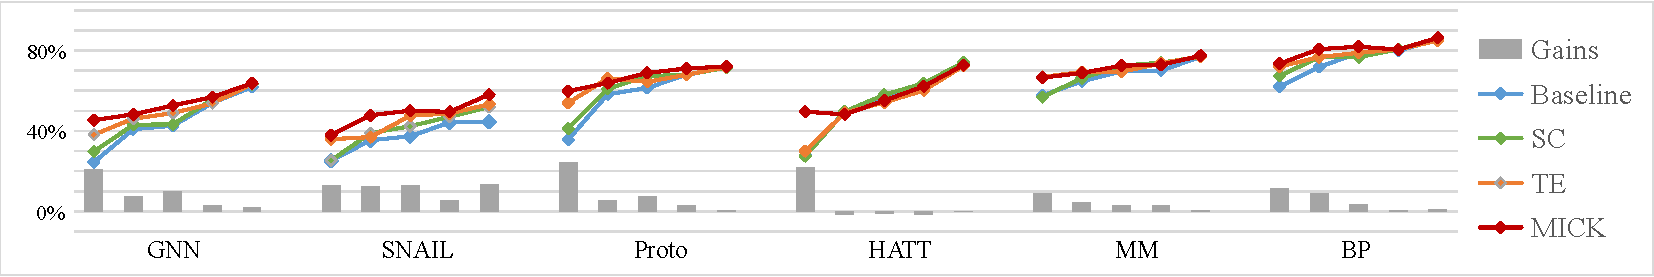
\includegraphics[width=\linewidth]{new51.pdf}
		%\caption{fig1}
	} \\
	\subfigure[5-way 5-shot]{
		\centering
		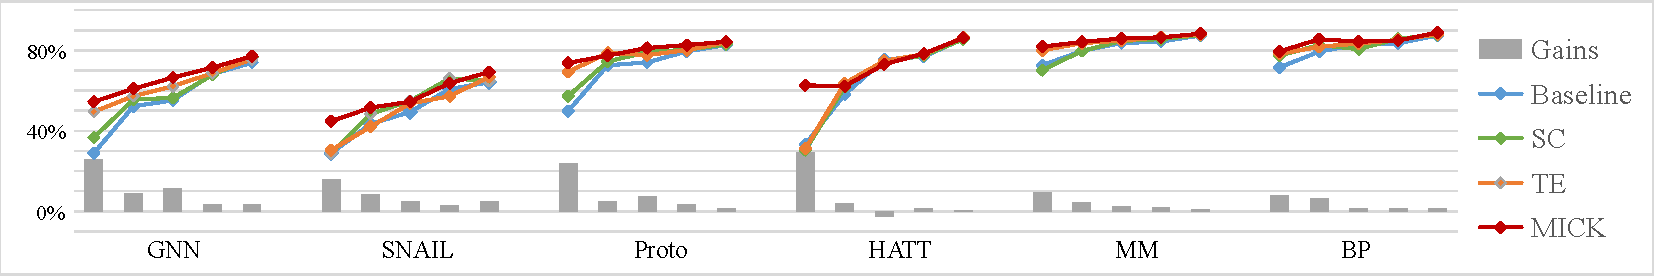
\includegraphics[width=\linewidth]{new55.pdf}
		%\caption{fig2}
	} \\%
	\subfigure[10-way 1-shot]{
		\centering
		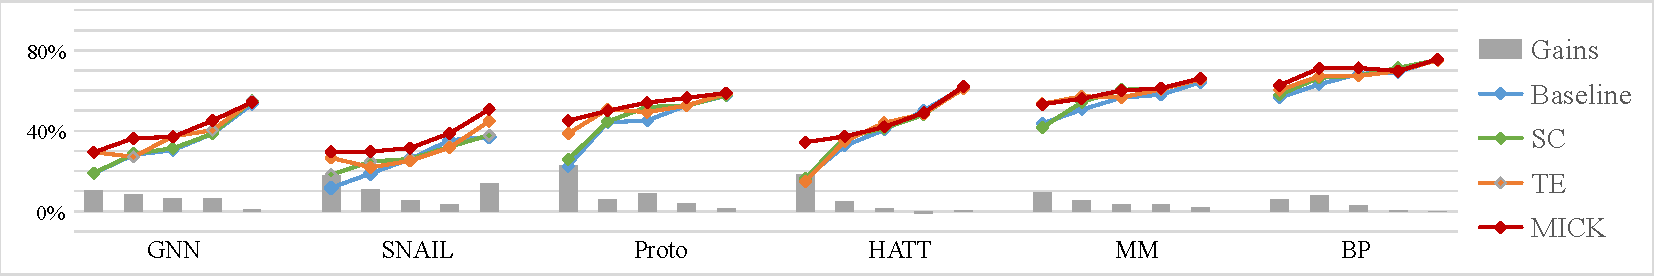
\includegraphics[width=\linewidth]{new101.pdf}
		%\caption{fig2}
	} \\
	\subfigure[10-way 5-shot]{
		\centering
		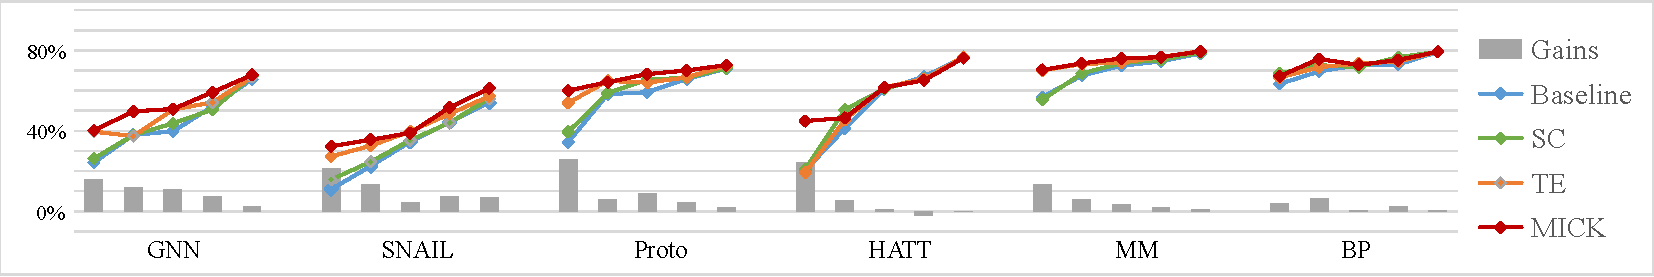
\includegraphics[width=\linewidth]{new105.pdf}
		%\caption{fig2}
	}%
	%\includegraphics[width=0.49\linewidth]{full_results.pdf}
	%%\caption{fig1}
	%}%
	%\subfigure[5-way 5-shot]{
	%\centering
	%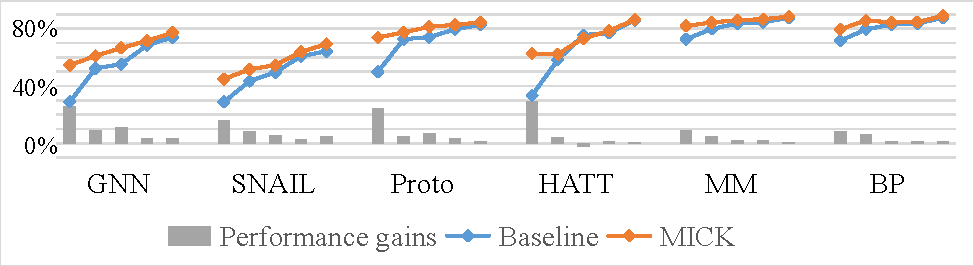
\includegraphics[width=0.49\linewidth]{55.pdf}
	%%\caption{fig2}
	%} \\%
	%\subfigure[10-way 1-shot]{
	%\centering
	%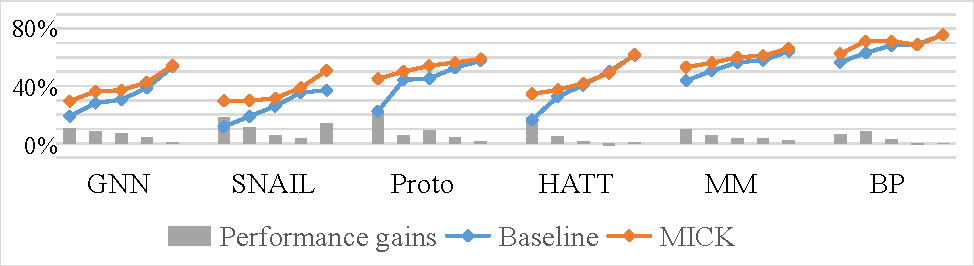
\includegraphics[width=0.49\linewidth]{101.pdf}
	%%\caption{fig2}
	%}%
	%\subfigure[10-way 5-shot]{
	%\centering
	%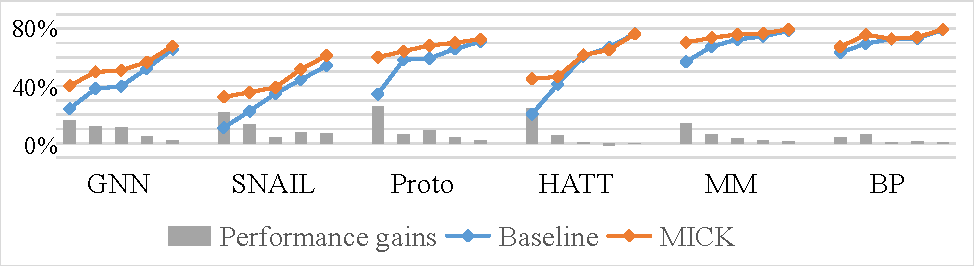
\includegraphics[width=0.49\linewidth]{105.pdf}
	%%\caption{fig2}
	%}%
	
	\centering
	\caption{Classification accuracy on FewRel validation set %with training data shrunken 
		under $N$-way $K$-shot configurations. Gains is the difference between MICK accuracy and baseline accuracy.
		For each group, from the left to the right, training data is shrunken to 0.22\%, 1.00\%, 2.23\%, 7.00\%, and 100.00\% of full training set size, respectively. For each shrunken training set, we apply baseline models and models with SC (Support Classifier individually), TE (Task Enrichment individually) and the whole MICK framework. Proto, HATT, MM, and BP stand for Prototypical Networks, Proto-HATT, MLMAN, and Bert-Pair, respectively.}
	\label{fig:analysis}
\end{figure*}


\subsection{Results and Analysis}
\label{results}
%\KZ{Put more analysis in this section. Make more observation and explain
%things more thoroughly.}
Here, we show the experimental results and analyze them from different aspects.

\subsubsection{With small training data}
To show the effectiveness of our MICK framework under small training data,
we apply it on each baseline model on
(1) FewRel dataset with training set shrunken to different extents, and (2) our proposed TinyRel-CM dataset.

\begin{table*}[th]
\centering
\small
\caption{Classification accuracy (\%) on TinyRel-CM dataset under
	$N$-way $K$-shot configuration.
	% For each cell, $K$=5, 10, and 15 from the top row to the bottom row. 
	D, S, F, and U stand for Disease, Symptom, Food, and nUtrient, respectively.
	Proto, HATT, MM, and BP stand for Prototypical Networks, Proto-HATT, MLMAN, and Bert-Pair, respectively.
	Gray numbers indicate the accuracy is lower than baseline.}
%Meta Networks, SNAIL, GNN, SNAIL and Proto-HATT require the number of classes while training and testing to be equal. So a model is trained with N way tasks to perform N way tests. For SNAIL, the number of instances per relation while training and testing need to be equal. So a model is trained with K shot tasks to perform K shot test tasks.}
\label{FRMresult}
\begin{tabular}{|c|c|cccccc|cccccc|}
\hline
\textbf{Method} & &\multicolumn{6}{c|}{\emph{Baseline}} &\multicolumn{6}{c|}{\emph{+SupportClassifier}} \\ \hline
&\textbf{Group} & D-D & D-S & D-F & D-U & F-U & S-F& D-D & D-S & D-F & D-U & F-U & S-F\\
&\textbf{(N)} & (5) & (2) & (6) & (6)& (2) & (6)& (5) & (2) & (6) & (6)& (2) & (6)\\ \hline
%\multirow{3}{*}{MetaN}      &&&&&& &&&&&& &&&&&& &&&&&&\\
% &&&&&& &&&&&& &&&&&& &&&&&& \\
%&&&&&& &&&&&& &&&&&& &&&&&& \\ \hline
\multirow{3}{*}{GNN}   & (K=~5~)   & 24.04&53.62 &34.15 &38.90 & 54.60& 32.45 &25.71&57.12&33.11&40.23&\textcolor[rgb]{0.45,0.45,0.45}{53.20}&34.51 \\
 & (K=10) & 26.05& 53.73&37.54 &44.02 &\textbf{55.53} &35.45 &\textbf{27.96}&57.35&37.44&43.87&\textcolor[rgb]{0.45,0.45,0.45}{54.85}&\textbf{38.39} \\
 & (K=15) & 26.94& 54.30&38.36 &45.12 &55.45 &37.43 &\textbf{28.36}&61.25&39.18&47.57&\textcolor[rgb]{0.45,0.45,0.45}{55.10}&\textbf{40.37}\\ \hline
\multirow{3}{*}{SNAIL}
 & (K=~5~) &21.74 & 50.00 &17.78 &25.98 & 47.96& 25.38     &23.64&53.90&27.28&27.60&53.15&25.88\\
  & (K=10) & 19.49 & 53.57&27.55 &22.96 &51.63 &22.51      &23.98&56.65&27.76&30.10&54.60&26.10 \\
 & (K=15) & 21.94& 51.62&20.03 &18.21 &50.33 &21.38         &23.12&\textbf{57.40}&27.72&31.43&\textbf{56.35}&25.40\\ \hline
\multirow{3}{*}{Proto}      & (K=~5~)  & 30.03&63.27 &31.35 &33.95 & 54.99& 26.97 &28.99 &\textbf{69.56} &33.57 & 43.78&56.49 &36.81\\
 & (K=10) & 31.68& 67.22&34.09 &36.27 &56.78 &29.18 &32.35 &\textbf{72.54} &36.10 & 47.78& 58.13&39.04\\
 & (K=15) & 33.80& 70.29&34.57 &37.41 &57.03 &29.72 &34.82 &\textbf{72.79} &36.96 &\textbf{50.03} &\textbf{ 60.09} &40.09\\ \hline

% D-D | D-S | D-F | D-U | F-U | S-F %
\multirow{3}{*}{HATT}
 & (K=~5~) &29.67&59.27&40.13&40.19&65.20&41.67  % baseline	5
&36.39&71.45&40.83&\textbf{54.17}&70.09&43.33 \\% cls + data  5
% -------
 & (K=10) &34.50&59.77&39.17&48.33&67.50&43.57  % baseline    10
&40.10&\textbf{71.24}&45.34&50.83&73.33&\textbf{49.17} \\% cls + data  10
% -------
 & (K=15) &39.01&63.75&37.41&\textbf{56.67}&66.25&37.13  % baseline	15
&43.05&77.09&44.17&\textcolor[rgb]{0.45,0.45,0.45}{51.67}&\textcolor[rgb]{0.45,0.45,0.45}{63.75}&45.92  % cls			15
\\% cls + data  15
\hline

\multirow{3}{*}{MM}   & (K=~5~)     &31.22 &60.58 &44.97 &47.11 &61.04 &44.78 &33.48 &62.34 & \textcolor[rgb]{0.45,0.45,0.45}{44.93}&49.49 &62.40 &45.90\\
 & (K=10) & 36.66&64.96 &49.44 &52.49 &66.68 &50.57 &38.89 & 67.30& 50.09& 54.09&68.39 &50.77\\
 & (K=15) & 40.65&68.14 &52.44 &56.00 &70.32 &53.13 &43.05 & 69.41&53.82 &57.23 &72.02 & \textcolor[rgb]{0.45,0.45,0.45}{52.87}\\ \hline
\multirow{3}{*}{BP}  & (K=~5~)    & 23.61&53.48 &46.02 &42.03 & 54.17& 46.18&   24.60 &\textcolor[rgb]{0.45,0.45,0.45}{53.98}&50.49 &\textbf{43.28}&\textbf{63.33}&48.75 \\
 & (K=10) & 24.17& 56.95&49.52 &44.37 &59.72 &48.96 &26.69&\textcolor[rgb]{0.45,0.45,0.45}{55.05} &53.60 &\textbf{46.13}&\textbf{66.70} &51.63  \\
 & (K=15) & 25.80& 54.15&50.38 &45.16 &59.33 &48.78 &27.29 &56.65 &54.22&\textbf{47.81} &67.55 &52.48 \\ \hline
%\multirow{3}{*}{BP2}      & \emph{K=~~5} & 21.83&52.52 &28.73 &30.68 & 54.69& 27.79 &&&&&& &&&&&& &&&&&&\\
%& \emph{K=10} & 22.15& 53.34&32.15 &34.52 &55.20 &30.95 &&&&&& &&&&&& &&&&&&\\
%& \emph{K=15} & 21.56& 54.83&33.74 &36.95 &55.99 &33.00 &&&&&& &&&&&& &&&&&&\\ \hline
%\hline

\textbf{Method} & & \multicolumn{6}{c|}{\emph{+TaskEnrich}} &\multicolumn{6}{c|}{\emph{+SupportClassifier\&TaskEnrich}} \\ \hline
& \textbf{Group} & D-D & D-S & D-F & D-U & F-U & S-F& D-D & D-S & D-F & D-U & F-U & S-F\\
& \textbf{(N)} & (5) & (2) & (6) & (6)& (2) & (6)& (5) & (2) & (6) & (6)& (2) & (6)\\ \hline
\multirow{3}{*}{GNN}
 & (K=~5~) & 24.59&\textcolor[rgb]{0.45,0.45,0.45}{51.20}&\textcolor[rgb]{0.45,0.45,0.45}{33.28}&40.76&54.62&35.36 &\textbf{26.02}&\textbf{66.22}&\textbf{37.48}&\textbf{44.47}&\textbf{55.02}&\textbf{37.13} \\
 & (K=10) &26.85&56.05&37.56&44.90&\textcolor[rgb]{0.45,0.45,0.45}{54.12}&37.69 &27.66&\textbf{58.75}&\textbf{37.88}&\textbf{45.15}&\textcolor[rgb]{0.45,0.45,0.45}{53.42}&37.85 \\
 & (K=15) &27.71&58.55&40.42&49.43&56.35&40.13 &27.40&\textbf{70.10}&\textbf{43.25}&\textbf{51.40}&\textbf{56.45}&40.03 \\ \hline
\multirow{3}{*}{SNAIL}
 & (K=~5~) &22.43&53.95&25.17&\textbf{29.05}&51.30&27.27&\textbf{24.64}&\textbf{58.55}&\textbf{28.57}&27.08&\textbf{53.30}&\textbf{27.88} \\
 & (K=10) &22.79&\textcolor[rgb]{0.45,0.45,0.45}{51.98}&\textbf{30.67}&\textcolor[rgb]{0.45,0.45,0.45}{22.13}&53.15&23.03         &\textbf{27.38}&\textbf{57.12}&\textbf{27.85}&\textbf{33.50}&\textbf{55.60}&\textbf{30.52} \\
 & (K=15) &\textcolor[rgb]{0.45,0.45,0.45}{21.54}&53.10&20.77&\textbf{20.35}&52.00&23.30     &\textbf{23.84}& 56.70&\textbf{30.63}&\textbf{35.75}&54.30&\textbf{30.43} \\ \hline

\multirow{3}{*}{Proto}
 & (K=~5~) &31.40 &69.22 &32.13& 34.22&55.34&30.34&\textbf{31.50} &68.79 &\textbf{34.36} & \textbf{44.76} &\textbf{57.43}&\textbf{40.36} \\ 
 & (K=10) &34.80 &72.34 &34.51&36.58&57.29&33.81&\textbf{35.45} &71.37 &\textbf{37.11} & \textbf{48.28}&\textbf{58.71}&\textbf{43.55} \\
 & (K=15) &36.97 &71.62 &35.76 &37.79 &57.74&34.49&\textbf{38.28} &72.62 &\textbf{37.90} &49.58 &60.00&\textbf{44.97} \\ \hline

\multirow{3}{*}{HATT}
 & (K=~5~) &33.70&67.50&41.67&43.33&65.62&\textcolor[rgb]{0.45,0.45,0.45}{38.33} &\textbf{38.21}&\textbf{75.00}&\textbf{46.67}&49.17&\textbf{73.75}&\textbf{44.17} \\
 & (K=10) &38.98&68.75&40.13&48.75&\textcolor[rgb]{0.45,0.45,0.45}{60.92}&46.67  % data        10
&\textbf{44.45}&70.23&\textbf{49.37}&\textbf{51.67}&\textbf{75.00}&44.47 \\
 & (K=15) &40.39&72.31&43.84&\textcolor[rgb]{0.45,0.45,0.45}{55.83}&70.51&43.33  % data		15
&\textbf{49.61}&\textbf{80.41}&\textbf{44.33}&\textcolor[rgb]{0.45,0.45,0.45}{55.81}&\textbf{72.58}&\textbf{49.17} \\ \hline

\multirow{3}{*}{MM}
 & (K=~5~) &36.05 & \textbf{64.98}& 45.24&50.03 &61.34 & 46.82&\textbf{38.17} &64.68 & \textbf{45.32}& \textbf{51.30}& \textbf{64.24}& \textbf{48.34} \\
 & (K=10) &42.04 & \textbf{70.02}& \textbf{50.83} &54.85 &67.57 &52.47&\textbf{44.89} &69.93 & 50.75& \textbf{56.60}& \textbf{70.79} &\textbf{53.69} \\ 
 & (K=15) &46.55& 71.95&54.18 &58.19 &72.01 &55.28&\textbf{49.23} & \textbf{72.41}& \textbf{54.25}& \textbf{59.67}& \textbf{74.58}& \textbf{56.67} \\ \hline

\multirow{3}{*}{BP}
 & (K=~5~) &25.25&\textbf{59.52}&48.49&\textcolor[rgb]{0.45,0.45,0.45}{40.32}&55.73&48.68 &\textbf{26.87}&58.35&\textbf{52.54}&\textcolor[rgb]{0.45,0.45,0.45}{39.48}&62.52&\textbf{49.95} \\
 & (K=10) &27.54&61.48&51.11&\textcolor[rgb]{0.45,0.45,0.45}{44.33}&60.15&51.56 &\textbf{28.19}&\textbf{62.32}&\textbf{55.86}&\textcolor[rgb]{0.45,0.45,0.45}{43.25}&66.38&\textbf{52.92} \\
 & (K=15) &28.29&\textbf{63.98}&52.18&47.32&61.02&53.36 &\textbf{29.25}&63.15&\textbf{57.60}&\textcolor[rgb]{0.45,0.45,0.45}{43.26}&\textbf{68.83}&\textbf{54.16} \\ \hline
\end{tabular}
\end{table*}


Figure \ref{fig:analysis} shows the performance comparison between baseline models and our framework given different amount of training data on FewRel dataset. 
Each subgraph contains 6 groups, one group for each baseline model. For each group, the training data size increases from the left to right. 
Here, we focus on the blue curves which present baseline accuracies, the red curves which present the MICK enhanced model accuracies, and the gray bars which present the performance gains that MICK brings.
As is illustrated, performance of models deteriorates with the decrease of training data size. For example, the prototypical networks achieves 57.53\% accuracy with full training data under 10-way 1-shot test tasks, but performs poorly with 22.30\% accuracy given only 0.22\% of full training data.
Our framework fits in situations where only small training data is available. As is shown in Figure \ref{fig:analysis}, with our methods, the less the training data, the more improvement the model tends to gain. This indicates the effectiveness of our framework under extremely small training data. While our methods only improve prototypical networks by 1.27\% accuracy with full training data under 10-way 1-shot test tasks, it leads to 22.74\% improvement given 0.22\% of full training data.
%When the input sentence contains multiple relation classes, model performance drops (by 14.14\% under 2.23\% full FewRel training data under 5-way 5-shot tasks using MLMAN). 

Table \ref{FRMresult} shows the experimental results on the TinyRel-CM dataset.
Our framework considerably improves model performance in most cases.
Strong baselines on FewRel dataset such as Bert-Pair do not perform well, partially because the TinyRel-CM dataset is more verbal and informal, thus quite distinct from BERT-Chinese's pretraining data (Chinese Wikipedia).

On both datasets, when the input sentence contains multiple relation classes, model performance drops. E.g., under 2.23\% full FewRel training data under 5-way 5-shot tasks using MLMAN, classification accuracy on relation class \emph{mother} decreases by 14.14\% when \emph{spouse} or \emph{child} appears as interference.

\subsubsection{With sufficient training data}

We use full training data from FewRel dataset and apply MICK framework on each baseline model.

Here, we focus on the rightmost blue points, red points and gray bars of each group in \figref{fig:analysis}, which present the baseline performance, MICK performance and performance gains brought by MICK under full FewRel training data. As is shown in \figref{fig:analysis}, on full FewRel dataset, in most cases, our framework achieves better performance than baseline models.
The framework brings more improvement for relatively poor baselines such as GNN and SNAIL (about 5\% accuracy) than strong baselines such as MLMAN and Bert-Pair (about 1\% accuracy). This is because our framework aims to help models learn better and doesn't change the core part of the models. Full training data is sufficient for strong baselines to train a good model, leaving limited room for improvement. 
%However, we show in \figref{fig:analysis} that by cutting down the training data size, the advantage of our framework is apparent.



% \subsubsection{FewRel dataset with reduced training data}
%Table \ref{FewRelval} shows the experimental results on the FewRel dataset. We either keep the original training set or shrink the training set to different extents and test on the validation set. Table \ref{FewRelval} illustrates the strength of our framework and data augmentation method since performance gains are attained in most cases. While the MSI framework keeps helping models to leaner better, data augmentation tends to be more effective when training data is quite limited.
%Figure \ref{fig:analysis} shows the performance gains on MLMAN using MSI framework and data augmentation. The less the training data, the more improvement the model gains, indicating that the MSI framework and data augmentation method's effectiveness under extremely limited training data.




\subsubsection{Ablation tests}

Here, we focus on the individual effects of support classifier and task enrichment on baseline models. %We facilitate baseline models with either MSI framework or data augmentation and compare the performance with both baseline models and models with

As is shown in Figure \ref{fig:analysis} and Table \ref{FRMresult}, in most cases, either adding support classifier or task enrichment improves performance for baseline models.
%and either removing support classifier or data augmentation leads to performance decrease from the models trained with both methods.
This illustrates that both support classifier and task enrichment contribute to better performance.

On FewRel dataset, we focus on the green and orange curves in \figref{fig:analysis}, which present the accuracies of applying support classifier or task enrichment individually.
% Support classifier
Support classifier generally brings more performance gains when less training data is given. This is because with small training data, baseline models fail to extract adequate knowledge while the support classifier helps with the knowledge learning process.
In some rare cases such as SNAIL under 5-way 1-shot and 5-way 5-shot scenarios with 0.22\% training data, adding support classifier leads to not much improvement. 
This is because support classifier guides models to extract more knowledge from very limited resources, while the extractable knowledge is restricted by the training set size and some of the knowledge is even useless.
Support classifier improves poor baselines such as GNN and SNAIL to a larger extent than strong ones such as MLMAN and Bert-Pair because the support classifier makes up for the insufficient learning ability for poor models while is icing on the cake for strong models. %with sufficient training data.

%TE
Task enrichment is much more helpful than support classifier under small training data (when training data is shrunken to less than 1.00\%). This is because task enrichment compensates for the lack of learning sources of basic knowledge such as basic rules and grammar when training data is quite limited.
Improvement of task enrichment is also more obvious on poor baselines than strong ones. Since poor models fail to master some of the basic knowledge brought in original training data, the introduction of cross-domain data not only brings extra basic knowledge but also helps models to master knowledge in original training data by providing more related data.
%provides more learning resources and help the models learn better about basic knowledge. 

Applying both support classifier and task enrichment achieves best performance in most cases, because the two methods complement each other. Support classifier extract useful information from original training data and cross-domain data, and task enrichment provide extra sources for the support classifier. %knowledge from both original training set and cross-domain data are fully extracted. 
In some cases, although adding either support classifier or task enrichment does not affect much, applying them together leads to a great improvement (e.g., HATT under 0.22\% training data).
%When applied together, support classifier leads to more gains when applied on task enriched models. Because cross-domain data may lead to noise while support classifier helps to choose what to learn.

%Both support classifier and task enrichment bring more performance gains for poor baselines such as GNN and SNAIL than strong ones such as MLMAN and Bert-Pair. 
%Support classifier is more powerful on poor models because the support classifier makes up for the insufficient learning ability for poor models while is icing on the cake for strong models with sufficient training data.
%Improvement of task enrichment is also more obvious on poor baselines than strong ones. Since poor models fail to master basic knowledge such as basic rules and grammar, the introduction of cross-domain knowledge provides more learning resources and help the models learn better about basic knowledge. While for strong models that already learn basic knowledge well, cross-domain task enrichment may bring in noise because of distinct data distributions. This is why sometimes task enrichment brings negative gains.
%stable on strong baselines while fluctuates on poor ones. This reflects the unstableness of poor baselines. With defects in learning ability, supplementary data brings harder tasks and may confuse poor models, and this is why sometimes data augmentation brings negative gains.

On TinyRel-CM dataset (\tabref{FRMresult}), %the improvement is more obvious with either support classifier or task enrichment than on FewRel dataset because of more room for progress.
task enrichment brings about similar improvements for all baselines due to small training data. Support classifier leads to more performance gains than task enrichment individually,
indicating TinyRel-CM dataset is more challenging (the relation classes are much more similar than FewRel dataset) and baseline models fail to extract sufficient useful knowledge.
%indicating model's learning ability is more essential than extra knowledge. 
Although task enrichment brings not much improvement or even negative effects in some cases, adding support classifier simultaneously tend to raise the accuracy to a large extent (up to 10\%). 
The reason is that with insufficient learning ability %(including strong baselines such as MLMAN and Bert-Pair under small data size \KZ{On the one hand you said insufficient learning ability, on the other
%hand you said strong baseline, contradiction?}),
(although baselines such as MLMAN and Bert-Pair are relatively strong, their learning ability is still insufficient with small training data),
cross-domain data alone sometimes introduces
noise and thus confuses the model. But with the additional support classifier
that improves learning ability, models are able to learn more useful
knowledge from cross-domain data.
%This is because with poor learning ability (although baselines such as MLMAN and Bert-Pair are strong on FewRel dataset, their learning ability is still unsatisfying under such small data size), cross-domain data sometimes make things tougher and may confuse the model, while with support classifier which improves learning ability, models are able to learn useful knowledge from cross-domain data.

On %both FewRel dataset (\tabref{FewRelvalAll}) and
TinyRel-CM dataset (\tabref{FRMresult}), few cases occur where adding both support classifier and task enrichment performs worse than adding only one of them
(e.g., Bert-Pair under group D-U, and prototypical networks under group D-S in TinyRel-CM dataset).
The main reason is that while adding the support classifier helps models learn more and better, the model occasionally tend to pay excessive attention to the distinctive distribution of the cross-domain data.
As is shown in the corresponding results, in the vast majority of cases, while adding support classifier on baseline models raises accuracy, adding support classifier on task enriched models brings less improvement or even bad effect. This indicates stronger learning ability owing to the support classifier, and the distraction caused by cross-domain data.

\begin{table}[ht]
	\centering
	\small
	\caption{Human evaluation result on TinyRel-CM dataset under 5-shot scenario.}
	\label{human}
	\begin{tabular}{|c|cccccc|}
		\hline
		\textbf{Group} & D-D & D-S & D-F & D-U & F-U & S-F \\
		\textbf{(N)} & (5) & (2) & (6) & (6) & (2) & (6) \\ \hline
		\textbf{Acc(\%)} & 92.65 &96.53 & 86.93 & 91.77 & 96.71& 84.97\\ \hline
	\end{tabular}
\end{table}

\subsubsection{Dataset analysis}
Our TinyRel-CM dataset is a challenging task.
We human evaluate the dataset and results are illustrated in Table \ref{human}.
During the human-evaluation process, under $N$-way $K$-shot scenario, we provide instances of $N$ relation classes with $K$ instances per relation class. We use labels $1$ to $N$ to name the relation classes instead of their real names. A person is required to classify a new coming instance into one of the $N$ classes. 
We only evaluate the TinyRel-CM dataset under 5-shot scenarios because 10-shot and 15-shot tasks are too easy for human.
Three volunteers participated in the human evaluation process and we take the average accuracy as the final result.

Comparing Table \ref{FRMresult} and Table \ref{human}, the performance of state-of-the-art models is still far worse than human performance, indicating the TinyRel-CM dataset is a challenging task.


%Our TinyRel-CM dataset is more challenging than FewRel dataset.
%The TinyRel-CM dataset has two major difficulties.
%One is the tiny training data size. As is shown in \figref{fig:analysis}, as the training data shrinks, the performance of each model drops evidently. This indicates the less the training data, the more challenging the task becomes.
%
%The other difficulty is that, in TinyRel-CM dataset, given any test task, head and tail entity types of each relation class are the same. This makes the TinyRel-CM dataset more challenging than FewRel dataset even with similar amount of training data.
%Comparing \tabref{FRMresult} and \figref{fig:analysis}, taking baseline MLMAN as an example, MLMAN achieves over $80\%$ accuracy under 5-way 5-shot configuration with $2.23\%$ of full FewRel training data (20 classes with 50 instances per class), while only $31.22\%$ accuracy under 5-way 5-shot configuration (D-D group) with TinyRel-CM dataset (22 classes with 50 instances per class as training set).
%
%To confirm this issue, we choose relation class \emph{mother}, the head and tail entity types of which are \emph{PERSON1} and \emph{PERSON2}, in FewRel dataset as a sample for further analysis. We compute two accuracies: (1) Distinct entity type accuracy: classification accuracy of relation class \emph{mother} without any other candidate relation classes whose target entity types are \emph{PERSON1} and \emph{PERSON2}, and (2) Same entity type accuracy: classification accuracy of \emph{mother} where \emph{spouse} or \emph{child} is among the candidate classes in the same task. We do this analysis under three typical baseline models: prototypical networks, MLMAN and Bert-Pair. We conduct 5-way 5-shot test configuration under $2.23\%$ full training data (20 classes with 10 instances per class). Results are shown in \tabref{etypeanalysis}.  As is illustrated, the accuracy of \emph{mother} accompanied by \emph{spouse} or \emph{child} is much lower than the accuracy of \emph{mother} without same-entity-type classes, indicating shared target entity types among candidate classes brings challenge to models.
%Only two relation classes with the same target entity types raise such difficulty, not to mention the TinyRel-CM dataset where all candidate classes have common target entity types.
%
%\begin{table}[ht]
%\centering
%\small
%\caption{5-way 5-shot classification accuracy (\%) on relation class \emph{mother} in FewRel dataset.
%	Etype stands for Entity type.
%	%Distinct etype represents classification accuracy with other candidate classes that have distinct target entity types with \emph{mother}.
%	%Same etype represents classification accuracy where some candidate classes share same target entity types with \emph{mother}.
%	Proto, MM, and BP stand for Prototypical Networks, MLMAN, and Bert-Pair, respectively.}
%\label{etypeanalysis}
%\begin{tabular}{|c|p{56pt}<{\centering}|p{56pt}<{\centering}|}
%\hline
%\textbf{Method} &\textbf{Distinct Etype} & \textbf{Same Etype} \\ \hline
%Proto & 77.91 & 63.39 \\
%MM & 86.84 & 72.70 \\
%BP & 96.89& 54.67 \\ \hline
%\end{tabular}
%\end{table}


\input{RelatedWorkShort}
\section{Conclusions}
\label{sec:conclude}

%Accurately computing semantic similarity between terms is a challenging task in the applications of text analytics and text understanding.
We presented a lightweight, effective approach for
semantic similarity between terms with any multi-word expression.
It uses an isA semantic network extracted from large Web corpus
to provide contexts for the terms, employs a concept clustering algorithm
to disambiguate the senses of the input terms, and finally applies
a {\em max-max} similarity function to compute the similarity.
Extensive studies show that our clustering-based refined algorithm outperforms the state-of-the-art methods as well
as our basic algorithm in terms of pearson correlation coefficient on word pairs and MWE pairs.
The method is efficient enough to be applied on large scale data sets.
In our future work, we will focus on how to judge type checking more semantically and how to apply our method in the similarity calculation of short text.
%, and how to introduce the supervised algorithms instead of clustering methods for higher Pearson Correlation Coefficients.
%due to its lower time cost in the calculation of semantic similarity between terms. {\color{red} However, how to learn a more
%robust similarity function
% instead of a simple Max-Max similarity function, and how to introduce the supervised algorithms instead of clustering methods for higher Pearson
% Correlation Coefficients are still challenging and interesting issues for our
%future work.}

%\input{ThreeExamples}
%
% The following two commands are all you need in the
% initial runs of your .tex file to
% produce the bibliography for the citations in your paper.
\bibliographystyle{abbrv}
\bibliography{context}  % sigproc.bib is the name of the Bibliography in this case
% You must have a proper ".bib" file
%  and remember to run:
% latex bibtex latex latex
% to resolve all references
%
% ACM needs 'a single self-contained file'!
%
%APPENDICES are optional
%\balancecolumns
%\appendix
%Appendix A
%\balancecolumns
% That's all folks!
%\end{multicols}
\end{document}
